\documentclass[12pt,a4paper,oneside]{report}             % Single-side
%\documentclass[11pt,a4paper,twoside,openright]{report}  % Duplex

\usepackage{ifxetex}
\ifxetex
  \usepackage{fontspec}
\else
  \usepackage[T1]{fontenc}
  \usepackage[utf8]{inputenc}
  \usepackage{lmodern}
\fi

\usepackage[magyar]{babel} % Alapértelmezés szerint utoljára definiált nyelv lesz aktív, de később külön beállítjuk az aktív nyelvet.

\usepackage{combelow}
\usepackage{newunicodechar}

\newunicodechar{Ș}{\cb{S}}
\newunicodechar{ș}{\cb{s}}
\newunicodechar{Ț}{\cb{T}}
\newunicodechar{ț}{\cb{t}}

\usepackage{cmap}
\usepackage{amsfonts,amsmath,amssymb} % Mathematical symbols.
\usepackage[ruled,boxed,resetcount,linesnumbered]{algorithm2e} % For pseudocodes.
\def\algorithmcfname{algoritmus}
\makeatletter
\renewcommand{\fnum@algocf}{\AlCapSty{\AlCapFnt\thealgocf.\nobreakspace\algorithmcfname}}
\makeatother

\usepackage{booktabs} % For publication quality tables for LaTeX
\usepackage{graphicx}
\usepackage{sidecap}

%\usepackage{fancyhdr}
%\usepackage{lastpage}

\usepackage{anysize}
\usepackage{sectsty}
\usepackage{setspace}  % Ettol a tablazatok, abrak, labjegyzetek maradnak 1-es sorkozzel!

% For hyperlinks in the generated document. 
\usepackage{color}
\usepackage{listings} % For source code snippets.

%\usepackage[amsmath,thmmarks]{ntheorem} % Theorem-like environments.

\usepackage[hang]{caption}
\usepackage{scrextend}

\usepackage{indentfirst}
\usepackage{pdfpages}

\usepackage{xfrac}
\usepackage{eurosym}

\usepackage{fullpage} % a margokra is lehessen irni

\newcommand{\vigyazat}{\marginpar{\textcolor{red}{\emph{Vigy\'azat!}}}}

\usepackage{tikz}
\usepackage{verbatim}
\usetikzlibrary{arrows,shapes}
\usetikzlibrary{positioning}
\tikzset{main node/.style={circle,fill=blue!20,draw,minimum size=1cm,inner sep=0pt},
}

%--------------------------------------------------------------------------------------
% Language configuration -- choose one
%--------------------------------------------------------------------------------------
%--------------------------------------------------------------------------------------
% Elnevezések
%--------------------------------------------------------------------------------------
\newcommand{\dolgozatnyelve}{\selectlanguage{magyar}}



\newcommand{\bsc}{Diplomadolgozat}
\newcommand{\msc}{Disszert\'aci\'os dolgozat}

\newcommand{\pelda}{Példa}
\newcommand{\definicio}{Definíció}
\newcommand{\tetel}{Tétel}

\newcommand{\bevezeto}{Bevezető}
\newcommand{\koszonetnyilvanitas}{Köszönetnyilvánítás}
\newcommand{\abrakjegyzeke}{Ábrák jegyzéke}
\newcommand{\tablazatokjegyzeke}{Táblázatok jegyzéke}
\newcommand{\irodalomjegyzek}{Irodalomjegyzék}
\newcommand{\fuggelek}{Függelék}


\newcommand{\englishParagraph}{
	\setlength{\parindent}{0em} % angol nyelvű dokumentumokban jellemző
	\setlength{\parskip}{0.5em} % angol nyelvű dokumentumokban jellemző
	\nonfrenchspacing
}

\newcommand{\hungarianParagraph}{
	\setlength{\parindent}{2em} % angol nyelvű dokumentumokban jellemző
	\setlength{\parskip}{0em}   % angol nyelvű dokumentumokban jellemző
	\frenchspacing
}

\newcommand{\defaultParagraph}{
	\hungarianParagraph
}  % Beállítások magyar nyelvű dolgozathoz

%--------------------------------------------------------------------------------------
% Main variables
%--------------------------------------------------------------------------------------



% Szak alapkepzes vagy mesteri
\newcommand{\szakHU}{SZOFTVERFEJLESZT\'ES SZAK} % SZOFTVERFEJLESZTES vagy INFORMATIKA SZAK
\newcommand{\szakRO}{SPECIALIZAREA DEZVOLTAREA APLICA\c TIILOR SOFTWARE} % SPECIALIZAREA DEZVOLTAREA APLICA\c TIILOR SOFTWARE vagy INFORMATIC\v A
\newcommand{\szakEN}{SOFTWARE ENGINEERING SPECIALIZATION} %SOFTWARE ENGINEERING SPECIALIZATION vagy COMPUTER SCIENCE SPECIALIZATION

\newcommand{\dolgozattipusHU}{MESTERI DISSZERT\'ACI\'O} % MESTERI DISSZERT\'ACI\'O vagy DIPLOMADOLGOZAT
\newcommand{\dolgozattipusRO}{TEZ\v A DE MASTERAT} %TEZA DE MASTERAT vagy  LUCRARE DE DIPLOM\v A
\newcommand{\dolgozattipusEN}{MASTER THESIS} % MASTER THESIS vagy BACHELOR THESIS
\newcommand{\szerzo}{Szerző neve} % Szerző neve
\newcommand{\temavezetoA}{T\'emavezet\H o neve} 


% Fokozatok

%Egyetemi tan\'ar/ Profesor universitar/Full Professor
%Egyetemi docens/ Conferențiar universitar/Associate professor
%Egyetemi adjunktus/Lector universitar sau Șef de lucrări /Lecturer
%Egyetemi tan\'arseg\'ed/Asistent universitar/Assistant professor


\newcommand{\temavezetoAfokozat}{Egyetemi tan\'ar}% Első konzulens neve
\newcommand{\temavezetoAfokozatRo}{Profesor universitar}
\newcommand{\temavezetoAfokozatEn}{Full Professor}
\newcommand{\temavezetoB}{} % Második konzulens neve; hagyd üresen, ha egy konzulensed van.
\newcommand{\cimHu}{A dolgozat c\'ime} % Cím
\newcommand{\cimRO}{Titlul lucr\v arii}
\newcommand{\cimEN}{Title of the Bachelor thesis}
\newcommand{\ev}{2021} %az aktualis ev

%--------------------------------------------------------------------------------------
% Page layout setup
%--------------------------------------------------------------------------------------
% we need to redefine the pagestyle plain
% another possibility is to use the body of this command without \fancypagestyle
% and use \pagestyle{fancy} but in that case the special pages
% (like the ToC, the References, and the Chapter pages)remain in plane style

\usepackage{smartdiagram}
\usepackage{tikz,pgf}
\usepackage{pgfplots}
\pgfplotsset{width=7cm,compat=1.8}
\usetikzlibrary{matrix,calc,shapes}

\tikzset{
	treenode/.style = {shape=rectangle, rounded corners, draw, anchor=center, text width=5em, align=center, top color=white, bottom color=blue!20,inner sep=1ex},
	decision/.style = {treenode, diamond, inner sep=0pt},
	root/.style = {treenode, font=\Large, bottom color=red!30},
	env/.style = {treenode, font=\ttfamily\normalsize},
	finish/.style = {root, bottom color=green!40},
	dummy/.style = {circle,draw}
}


\setcounter{secnumdepth}{0}
\sectionfont{\large\upshape\bfseries}
\setcounter{secnumdepth}{2}

\sloppy % Margón túllógó sorok tiltása.
\widowpenalty=10000 \clubpenalty=10000 %A fattyú- és árvasorok elkerülése
\def\hyph{-\penalty0\hskip0pt\relax} % Kötőjeles szavak elválasztásának engedélyezése


%--------------------------------------------------------------------------------------
% Setup hyperref package
%--------------------------------------------------------------------------------------
\usepackage{xcolor}
\definecolor{bluecite}{HTML}{0875b7}
\usepackage[unicode=true,
bookmarksopen={true},
pdffitwindow=true, 
colorlinks=true, 
linkcolor=bluecite, 
citecolor=bluecite, 
urlcolor=bluecite, 
hyperfootnotes=false, 
pdfstartview={FitH},
pdfpagemode= UseNone]{hyperref}


%--------------------------------------------------------------------------------------
% Set up listings
%--------------------------------------------------------------------------------------



\definecolor{codegreen}{rgb}{0,0.6,0}
\definecolor{codegray}{rgb}{0.5,0.5,0.5}
\definecolor{codepurple}{rgb}{0.58,0,0.82}
\definecolor{backcolour}{rgb}{0.95,0.95,0.92}




\definecolor{lightgray}{rgb}{0.95,0.95,0.95}
\definecolor{darkgreen}{RGB}{3,125,80}
\lstset{frame=tb,
	language=Matlab,
	aboveskip=3mm,
	belowskip=3mm,
	showstringspaces=false,
	columns=flexible,
	basicstyle={\small\ttfamily},
	numbers=none,
	numberstyle=\tiny\color{gray},
	keywordstyle=\color{blue},
	commentstyle=\color{codegreen},
	%stringstyle=\color{mauve},
	breaklines=true,
	breakatwhitespace=true,
	tabsize=3,
	backgroundcolor=\color{lightgray},
}
\def\lstlistingname{k\'odr\'eszlet}	


%--------------------------------------------------------------------------------------
% Set up theorem-like environments
%--------------------------------------------------------------------------------------
% Using ntheorem package -- see http://www.math.washington.edu/tex-archive/macros/latex/contrib/ntheorem/ntheorem.pdf
%\swapnumbers
%\theoremstyle{plain}
%\theoremseparator{.}
\newtheorem{example}{\pelda}[section]

%\theoremseparator{.}
%\theoremprework{\bigskip\hrule\medskip}
%\theorempostwork{\hrule\bigskip}
%\theorembodyfont{\upshape}
%\theoremsymbol{{\large \ensuremath{\centerdot}}}
\newtheorem{definition}{\definicio}[section]

%\theoremseparator{.}
%\theoremprework{\bigskip\hrule\medskip}
%\theorempostwork{\hrule\bigskip}
\newtheorem{theorem}{\tetel}[section]

\newtheorem{conclusion}{Következtetés}[section]


%--------------------------------------------------------------------------------------
% Some new commands and declarations
%--------------------------------------------------------------------------------------
\newcommand{\code}[1]{{\upshape\ttfamily\scriptsize\indent #1}}
\newcommand{\doi}[1]{DOI: \href{http://dx.doi.org/\detokenize{#1}}{\raggedright{\texttt{\detokenize{#1}}}}} % A hivatkozások közt így könnyebb DOI-t megadni.

\DeclareMathOperator*{\argmax}{arg\,max}
%\DeclareMathOperator*[1]{\floor}{arg\,max}
\DeclareMathOperator{\sign}{sgn}
\DeclareMathOperator{\rot}{rot}


%--------------------------------------------------------------------------------------
% Setup captions
%--------------------------------------------------------------------------------------

\captionsetup[figure]{
	width=.75\textwidth,
	aboveskip=10pt}
\renewcommand{\captionlabelfont}{\bf}
%\renewcommand{\captionfont}{\footnotesize\it}


%--------------------------------------------------------------------------------------
% Redefine reference style
%--------------------------------------------------------------------------------------
\newcommand{\figref}[1]{\ref{fig:#1}.}
\renewcommand{\eqref}[1]{(\ref{eq:#1})}
\newcommand{\listref}[1]{\ref{listing:#1}.}
\newcommand{\sectref}[1]{\ref{sect:#1}}
\newcommand{\tabref}[1]{\ref{tab:#1}.}





%--------------------------------------------------------------------------------------
% Table of contents and the main text
%--------------------------------------------------------------------------------------
\begin{document}
	
% CIMOLDALAK
%~~~~~~~~~~~~~~~~~~~~~~~~~~~~~~~~~~~~~~~~~~~~~~~~~~~~~~~~~~~~~~~~~~~~~~~~~~~~~~~~~~~~~~
	%--------------------------------------------------------------------------------------
%	A magyar cimoldal
%--------------------------------------------------------------------------------------
\begin{titlepage}
	\begin{center}
	
		\large{\bfseries SAPIENTIA ERDÉLYI MAGYAR TUDOMÁNYEGYETEM} \\
		\large{\bfseries MAROSVÁSÁRHELYI KAR,} \\
		\large{\bfseries \szakHU} \\[2.5cm]
			\begin{center}
			
\includegraphics[scale=2]{images/sapientia-hu}
		\end{center}
		\vspace{0.4cm}
		\Large{\Large  \cimHu}\\[0.8cm]
		\vspace{0.2cm}
		\textsc{\Large \bfseries \dolgozattipusHU}\\[2.5cm]
		
		{
			\large
		
			\renewcommand{\arraystretch}{0.85}
			\begin{tabular}{cc}
				 \makebox[6.5cm]{Témavezető:} & \makebox[6.5cm]{Végzős hallgató:} \\ \noalign{\smallskip}
				 \makebox[6.5cm]{\temavezetoA,} & \makebox[6.5cm]{\szerzo} \\ {\temavezetoAfokozat}
			\end{tabular}
		}
		
		\vfill
		{\large \bfseries \ev}
	\end{center}
\end{titlepage}
	%--------------------------------------------------------------------------------------
%	The title page RO
%--------------------------------------------------------------------------------------

\begin{titlepage}
	\begin{center}
	
		\large{\bfseries UNIVERSITATEA SAPIENTIA DIN CLUJ-NAPOCA} \\
		\large{\bfseries FACULTATEA DE ȘTIINȚE TEHNICE ȘI UMANISTE,} \\
		
		\large{\bfseries \szakRO} \\[2.5cm]
		
			\begin{center}
			
\includegraphics[scale=2]{images/sapientia-ro}
		\end{center}
		
		\vspace{0.4cm}
		
	
		
		\Large{\Large \cimRO}\\[0.8cm]
		\vspace{0.5cm}
		\textsc{\Large \bfseries \dolgozattipusRO}\\[2.5cm]
		
		{
			\large
		
			\renewcommand{\arraystretch}{0.85}
			\begin{tabular}{cc}
				 \makebox[6.5cm]{Coordonator științific:} & \makebox[6.5cm]{Absolvent:} \\ \noalign{\smallskip}
				 \makebox[6.5cm]{\temavezetoA,} & \makebox[6.5cm]{\szerzo} \\
				 {\temavezetoAfokozatRo}
			\end{tabular}
		}
		
		\vfill
		{\large \bfseries \ev}
	\end{center}
\end{titlepage}
	%--------------------------------------------------------------------------------------
%	The title page EN
%--------------------------------------------------------------------------------------

\begin{titlepage}
	\begin{center}
	
		\large{\bfseries SAPIENTIA HUNGARIAN UNIVERSITY OF TRANSYLVANIA} \\
		\large{\bfseries FACULTY OF TECHNICAL AND HUMAN SCIENCES} \\
		\large{\bfseries \szakEN} \\[2.5cm]
		
			\begin{center}
			
\includegraphics[scale=2]{images/sapientia-en}
		\end{center}
		\vspace{0.4cm}
		\Large{\Large  \cimEN}\\[0.8cm]
		\vspace{0.5cm}
		\textsc{\Large \bfseries \dolgozattipusEN}\\[2.5cm]
		
		{
			\large
	
			\renewcommand{\arraystretch}{0.85}
			\begin{tabular}{cc}
				 \makebox[6.5cm]{Scientific advisor:} & \makebox[6.5cm]{Student:} \\ \noalign{\smallskip}
				 \makebox[6.5cm]{\temavezetoA,} & \makebox[6.5cm]{\szerzo} \\
				 {\temavezetoAfokozatEn}
			\end{tabular}
		}
		
		\vfill
		{\large \bfseries \ev}
	\end{center}
\end{titlepage}
	
	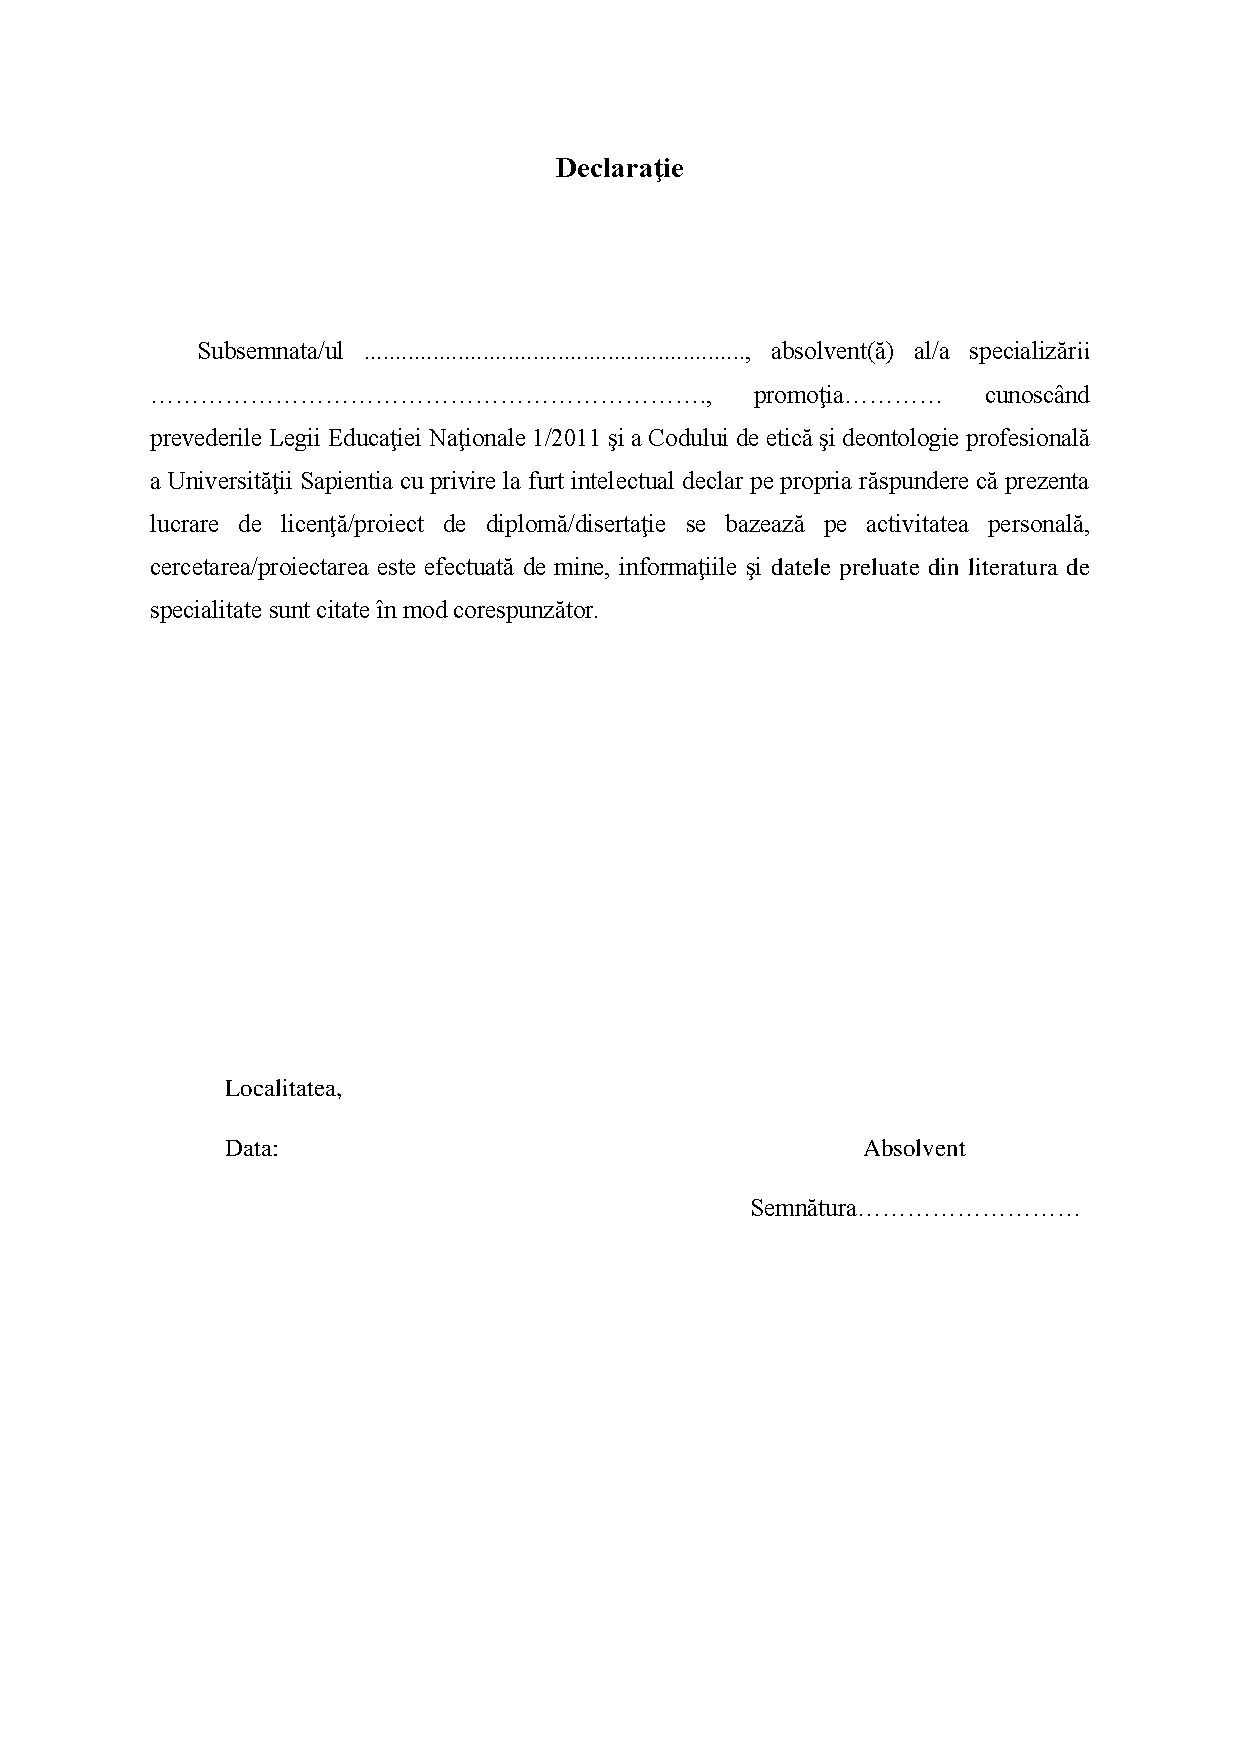
\includepdf[pages={1}]{content/Declaratie.pdf}
	\pagenumbering{gobble}

\selectlanguage{magyar}
\hungarianParagraph

%----------------------------------------------------------------------------
% Abstract in Hungarian
%----------------------------------------------------------------------------

\chapter*{Kivonat}

Dolgozatom témája a differenciálegyenletek megoldása különböző technológiák segítségével. Mint tudjuk a körülöttünk lévő világban szinte minden eseményt, jelenséget, problémát le tudunk írni differenciálegyenletek segítségével. Majd a kapott egyenletet vagy egyenleteket megoldjuk számítógép segítségével, valamilyen technológiát felhasználva.

Vannak olyan helyzetek az életben, amikor fontos, hogy ne csak pontosan, hanem a lehető leggyorsabban is meg tudjuk oldani ezeket az egyenleteket. Tehát számít az időtényező is, mert ezen akár emberi életek is múlhatnak. Ilyen jelllegű probléma lehet például valamilyen természeti katasztrófa előrejelzése vagy egy betegséggel kapcsolatban felmerülő jövőbeli kérdés megválaszolása. Ezekben az esetekben nagyon fontos lehet az, hogy a rendelkezésünkre álló szoftverek és programok közül, melyiket választjuk a probléma megoldására.

Jelen dolgozatomban arra a kérdésre keresem a választ, hogy milyen típusú szoftvert érdemes használni, ahhoz hogy az adott feladat egyenleteit a lehető leggyorsabban tudjuk megoldani. A szoftvereket két kategóriára osztom fel és így fogom megvizsgálni: olyan szoftverek melyek már léteznek és használhatóak differenciálegyenletek megoldására, valamint saját megvalósítású szoftverek.

A választott és megvalósított programokkal megoldatjuk ugyanazokat a feladatokat és minden esetben mérjük a futási időt. A teszteket megismételjük és átlagokat számítunk, hogy az eredmények még hitelesebbek legyenek. A végső eredményeket összehasonlítjuk és kiértékeljük.

Végül az eredmények alapján levonjuk a következtetéseket, hogy melyik módszert vagy technológiát érdemes használni vagy esetleg továbbfejleszteni a jövőben. Továbbá megállapítjuk azt is, hogyha egy adott technológiával nem érdemes tovább próbálkozni.
\vspace*{2cm}

\noindent \textbf{Kulcsszavak:} egy, kett\H o, h\'arom, n\'egy, max. \"ot.
\vfill
\selectlanguage{romanian}

%----------------------------------------------------------------------------
% Abstract in Romanian
%----------------------------------------------------------------------------
\chapter*{Rezumat}

Tema tezei este rezolvarea ecuațiilor diferențiale cu ajutorul diferitelor tehnologii. Cum știim în jurul nostru aproape toate acțiuniile și fenomenele ale naturii sau probleme date pot fi descrise cu ajutorul ecuației diferențiale. Ecuațiile primite vom rezolva cu ajutorul calculatorului, folosind oricare tehnologie.

Sunt situații în viață când este important nu numai exactitatea ci și rapiditatea rezolvării ecuațiilor. Deci contează și factorul timpului, fiindcă de aceasta pot depinde vieți omenești. Asemenea probleme pot fi de exemplu pronosticul catastrofelor naturale sau rezolvarea problemelor apărute în unele boli. În aceste cazuri este foarte importantă alegerea corectă a software-ului pentru rezolvarea problemei.

În teză caut răspunsul la folosirea software-ului potrivit pentru rezolvarea în mod cât mai rapid a problemei. Software-ele am împărțit în două grupuri: programuri care deja există și pot fi folosite pentru rezolvarea ecuațiilor și programe construite de mine.

Cu ajutorul programelor alese și rezolvate vom rezolva problema dată și măsurăm timpul necesar. Vom repeta testele și calculăm media pentru autentificarea rezultatelor. Facem compararea și evaluarea rezultatelor.

În final tragem concluzia ca care dintre tehnologii merită folosire sau dezvoltare. În plus constatăm în ce tehnologie nu merită să învestigăm.
\vspace*{2cm}


\noindent \textbf{Cuvinte de cheie:} egy, kett\H o, h\'arom, n\'egy, max. \"ot.

\vfill
\selectlanguage{english}
%\englishParagraph

%----------------------------------------------------------------------------
% Abstract in English
%----------------------------------------------------------------------------
\chapter*{Abstract}

The aim of my thesis is to solve differential equations using different technologies. We know that in the world around us, we can describe almost every
event, phenomenon using differential equations. We can then solve the given equation or system of equations with the help of a computer, using some technology.

There are situations in real life when it is necessary to solve the equations not only as  accurately but as quickly as possible. The time factor is also very important because human lives may also depend on it. Such a problem might be a natural disaster forecast or the need to urgently answer a disease related question. In these cases our choice of available software is critical in solving the problem.

In this thesis I aim to identify the best software for solving the problem as quickly as possible. I split the software into two groups: programs that already exist and which can be used to solve the equations, and programs that I have built.

With the help of the chosen and solved programs, we will solve the problem and measure the time taken to achieve this. We will repeat the tests and calculate the median for the authentication of the results. We compare and evaluate the results.

Finally, we reveal which technology is worth using or developing. In addition, we identify which technology is not worth investigating.

\vspace*{2cm}

\noindent \textbf{Keywords:} egy, kett\H o, h\'arom, n\'egy, max. \"ot.

\vfill
\dolgozatnyelve
\defaultParagraph
 
% Tartalomjegyzek
%~~~~~~~~~~~~~~~~~~~~~~~~~~~~~~~~~~~~~~~~~~~~~~~~~~~~~~~~~~~~~~~~~~~~~~~~~~~~~~~~~~~~~~
	\pagenumbering{arabic}
	\setcounter{page}{9}
	\tableofcontents\vfill

% A diplomadolgozat lenyegi resze
%~~~~~~~~~~~~~~~~~~~~~~~~~~~~~~~~~~~~~~~~~~~~~~~~~~~~~~~~~~~~~~~~~~~~~~~~~~~~~~~~~~~~~~

% ajánlott külön file-okba írni az egyes fejezeteket, ugyanis úgy jobban át lehet látni.



	%----------------------------------------------------------------------------
\chapter{Bevezető}%\addcontentsline{toc}{chapter}{Bevezető}
%----------------------------------------------------------------------------

Ez a fejezet mutatja be a dolgozat témáját, helyezi el a témát a szakterületen. Indokolni kell a témaválasztást, majd utalni a választott téma jelentőségére, az alkalmazott közelítésmódra, és a téma feldolgozásának gyakorlati hasznosságára. A bevezető szerepe, hogy meggyőzze az olvasókat, miért hasznos az elvégzett munka. 
A bevezető a következő kérdésekre ad választ:

\begin{itemize}
\item Mi a probléma?
\item Mit szeretne a szerző elérni?
\item Mit sikerült megvalósítani?
\end{itemize}


Fontos, hogy a fejezet fogalmazza meg a munka célkitűzéseit, esetleg térjen ki arra is, hogy milyen módszerekkel kívánt a szerző választ kapni a felvetett kérdésekre. 


\section{P\'elda fejezet}


Felmerülhet bennünk a kérdés, hogy mi is az a differenciálegyenlet és hogy egyáltalán mire jó, vagy hol használhatjuk fel? Röviden összefoglalva a differenciálegyenlet egy olyan egyenlet, amelyben az ismeretlen egy függvény és az egyenlet tartalmazza a függvény valamilyen rendű deriváltját is. Tehát nem ismerjük a konkrét függvényt, csak annak változását különböző időpillanatokban.

Ha jobban belegondolunk a mindennapi életben is rengeteg ilyen esemény, jelenség, folyamat, stb. vesz körül, amit csak megfigyelni tudunk, de nem tudjuk konkrétan leírni matematikai vagy fizikai képletekkel. Itt jönnek képbe a differenciálegyenletek, az előbbiekben elmondottak alapján tökéletesen alakalmasak az ilyen jellegű problémák felírására, modellezésére. Egy egyszerű kis példa az az eset, amikor a sütőből kiveszünk egy forró süteményt és ennek a kihülését szeretnénk valamilyen módon megviszgálni. Ez úgy lehetséges, hogy különböző időpillanatokban megmérjük a sütemény hőmérsékletét és lejegyezzük, majd ezekből az előzetes ismeretekből felállítjuk a differenciálegyenletünket. Miután megvan az egyenletünk (modellünk) már csak meg kell oldani. Mai fejlett világunkban ezt már nem papíron analitikus módszerekkel végezzük, azért sem, mert sok esetben nem is lehetséges kézzel megoldani az egyenleteket, ezért segítségül hívjuk a számítógépet és numerikus szamításokkal próbáljuk megoldani az adott problémát.

A valós életben vannak sokkal bonyolultabb esetek is, amikor nem ilyen egyszerű felírni, megalkotni vagy megoldani a probléma modelljét (figyelembe kell venni számos más környezeti behatást, tényezőt). Emellett nagyon fontos az is, hogy egy adott problémát milyen gyorsan és hatékonyan tudunk megoldani a mai számítógépek és technológiák segítségével. Dolgozatom témájának megválasztásánál is ez a feladat keltette fel leginkább az érdeklődésem, hogy hogyan lehet azokat a bizonyos egyenleteket a leggyorsabban megoldani. Vannak olyan esetek vagy problémák, ahol a gyorsaság és hatékonyság elengedhetetlen. Például egy súlyos betegség vagy természeti katasztrófa előrejelzésénél fontos, hogy a modellünket a lehető leggyorsabban megoldjuk és még időben tudjuk jelezni ha baj van. Ezekben az esetekben nagyon fontos, hogy az adott modellt megoldó szoftverünk milyen technológiákkal és módszerekkel van megvalósítva.
%\vigyazat

A doldozat további részében ismertetem a differenciálegyenletek numerikus megoldásának elméleti alapjait, majd olyan konkrét modelleket vizsgálunk meg, amelyek esetében fontos az időtényező. Továbbá bemutatom a különbző technológiákkal megvalósított szoftvereket, megvizsgáljuk ezeknek a hatékonyságát külön-külön és egymáshoz képest is. Végül megpróbáljuk megtalálni a megvalósított szoftverek közül azt, amelyik a legjobban teljesít gyorsaság szempontjából a különböző tesztek során. %\vigyazat
\cite{Knuth}


	``Maxwell's equations'' are named for James Clark Maxwell and are as follow:
\begin{align}             
	\vec{\nabla} \cdot \vec{E} \quad &=\quad\frac{\rho}{\epsilon_0} &&\text{Gauss's Law} \label{eq:GL}\\      
	\vec{\nabla} \cdot \vec{B} \quad &=\quad 0 &&\text{Gauss's Law for Magnetism} \label{eq:GLM}\\
	\vec{\nabla} \times \vec{E} \quad &=\hspace{10pt}-\frac{\partial{\vec{B}}}{\partial{t}} &&\text{Faraday's Law of Induction} \label{eq:FL}\\ 
	\vec{\nabla} \times \vec{B} \quad &=\quad \mu_0\left( \epsilon_0\frac{\partial{\vec{E}}}{\partial{t}}+\vec{J}\right) &&\text{Ampere's Circuital Law} \label{eq:ACL}
\end{align}
Equations (\ref{eq:GL}), (\ref{eq:GLM}), (\ref{eq:FL}), and (\ref{eq:ACL}) are some of the most important in Physics.


	%----------------------------------------------------------------------------
\chapter{Elméleti megalapozás és szakirodalmi tanulmány} \label{fejezet3}
%----------------------------------------------------------------------------

A szakirodalmi tanulmány a téma pontos körülhatárolása érdekében végzett dokumentálás. Ez a fejezet tartalmazza az irodalomkutatást, a hasonló alkalmazások, megoldások rövid ismertetőjét, amelyek már léteznek. Ugyancsak ide kerül azoknak a technológiáknak, elméleti ismereteknek a rövid bemutatása, amelyek szükségesek a megvalósítás megértéséhez.
Figyelem: ez egy szintézis kell legyen, nem pedig összeollózott szöveg. Mindennek az eredetét bibliográfiai hivatkozással kell jelezni, a szó szerint átvett részeket idézőjelbe kell tenni a forrás megjelölésével. A dolgozatokat plágium detektáló szoftverrel ellenőrzik.
Az irodalmi áttekintés a szakirodalom az adott területének kritikus, letisztázó elemzése, mely összegzésen, osztályozáson és összehasonlításon alapszik. Korábban közölt adatokat dolgoz fel. Érdemes a témában survey/review címszó alatt közölt cikkeket keresni. Választ ad a következő kérdésekre: 
Létezik-e egyáltalán megoldás vagy megoldások a felvetett problémára? Melyik az eddigi  legjobb megoldás?
Melyek a létező megoldások fő korlátai? 




Kétféle szakdolgozatot különböztetünk meg: kutatás-fejlesztés, szoftverfejlesztés.
Amennyiben a dolgozat \textbf{kutatás-fejlesztés} kategóriába esik (pl. képfeldolgozás, jelfeldolgozás, matematikai modellezés, stb. ) akkor a hangsúlyt az \textit{elméleti vonalra} kell fektetni, pl. milyen elméleti megközelítések léteznek, ezek korlátai, illetve hol lehet a létező megoldásokon javítani.

\textbf{Szoftverfejlesztés}sel kapcsolatos dolgozat esetében (mobilalkalmazás, webes alkalmazás, játékfejlesztés) a hangsúlyt a már \textit{létező szoftverek, technologiák összehasonlítására} kell fektetni. 




\section {Beépített szoftverek, könyvtárak}

Dolgozatom ezen részében előszőr vizsgáljunk meg olyan beépített differenciálegyenlet megoldó szoftvereket, melyeket már megemlítettem. Ezek közül én a Matlab és a Boost - Odeint beépített programját használtam és vizsgáltam meg. Mindkét esetben közönséges differenciálegyenletek (ODE) megoldására, az előre megírt algoritmus segítségével, melynek hátterében természetesen a Dormand-Prince módszer áll.


	\begin{align}
	x&=1+1+1+1\\
	&=4.
\end{align}

	\begin{align}
	y&=mx+b\nonumber\\
	z&=nw+c.
\end{align}

			\begin{align}
	\int_0^1\sum_a^b\prod_\alpha^\beta.
\end{align}
	\begin{align*}
	\frac{12}{34}.
\end{align*}



\begin{definition}
	Legyen $\left(X,d\right)$ \'es $\left(Y,\rho\right)$ k\'et metrikus
	t\'er, legyen $T:X\to Y$ egy lek\'epez\'es. Azt mondjuk, hogy a $T$ lek\'epez\'es
	Lipschitz tulajdons\'ag\'u, ha l\'etezik egy olyan $L>0$ sz\'am amelyre 
	\[
	\rho\left(Tx,Ty\right)\leq Ld(x,y)\;\forall x,y\in X.
	\]
	Az L sz\'amot Lipschitz \'alland\'onak nevezz\"uk.
\end{definition}


Ha $T:X\to Y$ lek\'epez\'es Lipschitz tulajdons\'ag\'u, \'es az $L<1$ akkor
a $T$ oper\'atort \textbf{kontrakci\'onak} nevezz\"uk. Azt mondjuk, hogy
$x^{*}\in X$ fixpontja a $T$ oper\'atornak ha 
\[
Tx^{*}=x^{*}.
\]
\begin{theorem}{Banach f\'ele fixpontt\'etel}
	Legyen $\left(X,d\right)$ teljes metrikus t\'er \'es $T:X\to X$ lek\'epez\'es
	egy kontrakci\'o az $L<1$ \'alland\'oval. Ekkor igazak a k\"ovetkez\H{o}
	\'all\'it\'asok:
	\begin{enumerate}
		\item $T$-nek egy \'es csakis egy $x^{*}$ fixpontja.
		\item B\'arhogy v\'alasztunk meg egy $x_{0}\in X$ elemet, a $x_{k+1}=Tx_{k}$
		sorozat konvergens \'es $Tx_{k}\to x^{*},$ ahol $k$ term\'eszetes sz\'am.
		\item Igaz, hogy 
		\[
		d\left(x_{k},x^{*}\right)\leq\frac{L^{k}}{1-L}d(x_{0},Tx_{0}).
		\]
	\end{enumerate}
\end{theorem}



\subsection {Matlab - \href{https://www.mathworks.com/help/matlab/ref/ode45.html}{ode45}} \label{MatlabOde45}

A Matlab egy programcsomag és egyben egy technikai nyelv is, mely magas szinten lehetőséget biztosít számítások elvégzésére, modellezésre, szimulációra, megjelenítésre, vizualizációra és számos más hasznos mérnöki munka elvégzésére. Esetünkben a legfontosabb, hogy könnyedén tudunk közönséges differenciálegyenleteket megoldani az ode45 program segítségével. Emellett az eredményeket egy jól megtervezett felületen ki is tudjuk ábrázolni. Az alábbi példában jól látható, hogy milyen egyszerű és kényelmes a használata:

\begin{lstlisting}[caption={Matlab példakód diff. egyenlet megoldására.}, captionpos=b]
	f = @(t,y) y;
	t = [0 10];
	y0 = 1.0;
	ode45(f, t, y0);
	plot(t, y(:));
\end{lstlisting}


A fenti bemenetre $ n = 100 $ - szor lefuttattuk az algoritmust és a következő időeredményeket kaptuk:
\begin{itemize}
	\item Futási idők \textbf{átlaga}: $ 0.0043 $ sec
	\item Futási idők \textbf{minimuma}: $ 0.0026 $ sec
	\item Futási idők \textbf{maximuma}: $ 0.1504 $ sec
\end{itemize}




\begin{center}
\smartdiagram[flow diagram:horizontal]{Edit,
	\LaTeX, Bib\TeX/ biber, make\-index, \LaTeX}
\end{center}

\subsection {Boost - \href{http://headmyshoulder.github.io/odeint-v2/}{Odeint}} \label{BoostOdeint}

Egy másik előre megírt közönséges differenciálegyenlet megoldó a Boost könyvtárcsomag Odeint nevezetű könyvtára. Ez egy modern C++ nyelven írt csomag, lényeges jellemzői, hogy \textbf{nagy teljesítményre} képes és \textbf{nagyon magas szinten} (absztraktan - Template Metaprogramming) van megírva, így \textbf{rugalmas} és könnyen integrálható különböző rendszerekbe. Emellett rugalmas a bementi adatok típusát illetően is. Ugyanakkor jó tudni, hogy ez a nagyon absztrakt megvalósítás hátrány is lehet, mert bizonyos esetekben nagyon nehéz megérteni vagy megoldani egy felmerülő problémát. Most lássunk egy egyszerű példát a használatára:

\begin{lstlisting}[caption={Odeint példakód.}, captionpos=b, language = C++]
#include <iostream>
#include <boost/numeric/odeint.hpp>

using namespace std;
using namespace boost::numeric::odeint;

typedef runge_kutta_dopri5<double> stepper_type;

void rhs( const double x , double &dxdt , const double t ) {
	dxdt = 3.0/(2.0*t*t) + x/(2.0*t);
}

void write_cout( const double &x , const double t ) {
	cout << t << '\t' << x << endl;
}

int main() {
	double x = 0.0;    
	integrate_adaptive( make_controlled( 1E-12 , 1E-12 , stepper_type() ) ,
	rhs , x , 1.0 , 10.0 , 0.1 , write_cout );
}
\end{lstlisting}
\pagebreak
Az előző kódrészlet eredménye a következő:



\begin{itemize}
	\item Futási idők \textbf{átlaga}: $ 0.0989 $ sec
	\item Futási idők \textbf{minimuma}: $ 0.09 $ sec
	\item Futási idők \textbf{maximuma}: $ 0.099 $ sec
\end{itemize}

\section {P\'elda k\'odr\'eszletre} \label{fejezet3_2}

\begin{lstlisting}[caption={Matlab kód ode45 használata nélkül.}, captionpos=b, language = Matlab]
function [yy, tt, timeSpent] = fun_dopri45(f, y0, t0, tf, tolerance)
	...
	while t < tf
		if (t+h >= tf)
			h = tf-t;
		end
		
		% Calculate k1, k2, ... , k7
		k1 = h*feval(f, t+h*C(1), y);
		k2 = h*feval(f, t+h*C(2), y + A2(1)*k1);
		...
		k7 = h*feval(f, t+h*C(7), y + A7(1)*k1 + A7(3)*k3 + ... + A7(6)*k6);
		
		% Calcaulate the next point
		yt = y + A7(1)*k1 + A7(3)*k3 + A7(4)*k4 + A7(5)*k5 + A7(6)*k6;
		% Calculate the error
		err = abs(E(1)*k1 + E(3)*k3 + ... + E(7)*k7);
		
		if max(err) < tolerance
			t = t + h;
			y = yt;
			...
		end
		
		% Calculate optimal step size
		scale = 1.25*(maxErr/tolerance)^(1/5);
		if scale > 0.2
			h = h / scale;
		else
			h = 5.0*h;
		end
	end
end
\end{lstlisting}





	%----------------------------------------------------------------------------
\chapter{A rendszer specifikációja}
%----------------------------------------------------------------------------



Ajánlott a \href{https://drive.google.com/file/d/1Fmg_N5Zov1e_GZzF8uGK2GAkMDoo0_vm/view?usp=sharing}{Volere template} átnézése: egyrészt ad egy keretet, másrészt rengeteg jó kérdést tesz fel, melyre csak válaszolni kell a mi projektünk esetében. Azokat a részeket, amelyek nem relevánsak, egyszerűen ki lehet hagyni.
Az UML diagramok készítésénél ajánlott a James Sugrue \'altal k\'esz\'itett útmutatót használni\footnote{\href{https://drive.google.com/drive/folders/1ocZsC26FMHKStwkEhZx8H4od6Mk3Deo3}{\'Utmutat\'o}}.


\section{Felhasználói követelmények}


Ide jönnek a használati esetek (use case diagram), és a hozzá tartozó leírás. Figyelem: itt csak felhasználói szemszögből tekintünk a rendszerre. A felhasználó nem ismeri a Python programozási nyelvet, sem a publikus kulcsszót. 






\section{Rendszerkövetelmények}

Itt már rendszer szemszög van előtérben. 

\begin{enumerate}
	\item[a)] \textbf{Funkcionális követelmények, mire képes a rendszer.} A fontosabb funkcionalitásokat egyenként kell részletezni. Erre használható az \href{https://www.businessanalystlearnings.com/blog/2013/9/30/the-3-step-guide-to-documenting-requirements-with-use-cases}{itt} látható sablon. Lehet aktivitás-, szekvencia-, illetve együttműködési diagramokat hasznáni.
	\item[b)] \textbf{Nem funkcionális követelmények, megszorítások.} Itt érdemes kiindulni a \href{https://cs.ccsu.edu/~stan/classes/CS410/notes16/04-Requirements.html}{Sommerville} csoportosításból: 
	
	\begin{itemize}
		\item Termékkel kapcsolatos követelmények (pl mennyi tárhelyre van szükség?), 
		\item Hány kérést tud kiszolgálni másodpercenként, 
		\item Szervezéssel kapcsolatos követelmények (pl. Milyen operációs rendszer, vagy milyen verziókövető rendszer?),
		\item Külső követelmények (pl GDPR).
	\end{itemize}
	
	
	
	
	
	
	
\end{enumerate}






\section {P\'elda}

A \ref{fejezet3}. fejezetben bemutattam két beépített, előre megvalósított szoftvert, melyek a Matlab ode45 programja és a Boost - Odeint könyvtár. Az elért eredmények és tesztek azt mutatják, hogy a Matlab ode45 differenciálegyenlet megoldója sokkal gyorsabb és hatékonyabb, mint az Odeint. Ha a tesztesetekben mért átlagidőket összehasonlítjuk láthatjuk (\ref{fejezet3_3}. alfejezet), hogy az ode45 $ 20-30 $ -szor gyorsabb a Odeintnél. Ez talán annak is köszönhető, hogy a Matlab egy nagyon komoly szoftver, amelynek programcsomagjain mérnökök és programozók százai  (vagy akár ezrei) dolgoznak, így természetes, hogy az algoritmusok jobban optimizáltak és hatékonyabbak az ingyenes szoftvereknél. A továbbiakban összegezzük, hogy a két technológiának milyen előnyei és hátrányai vannak vagy éppen miért érdemes/nem érdemes használni őket, l\'asd \cite{Lovasz}
\\ \\
\textbf{Matlab ode45 előnyei:}
\begin{itemize}
	\item nagyon egyszerű a használata, nem igényel komoly programozási ismereteket
	\item könnyű beépíteni és összekötni más Matlab programokkal
	\item a kapott eredményeket mátrix vagy vektor típusokban téríti vissza, ami könnyűvé teszi az eredmények további kezelését
	\item az eredményeket grafikus felületen azonnal meg tudjuk jeleníteni
	\item jobb eredményeket produkált, mint az Odeint
	\item jól dokumentált, sok példa van a használatára
\end{itemize}
\pagebreak
\textbf{Matlab ode45 hátrányai:}
\begin{itemize}
	\item komoly hátránya az Odeinttel szemben, hogy \textbf{fizetni kell a használatáért}
	\item nagyon sok memóriát használ, komolyan igénybeveszi a számítógép erőforrásait
\end{itemize}
\textbf{Odeint előnyei:}
\begin{itemize}
	\item ingyenes és nyílt forráskódú, használható személyi és kereskedelmi célokra egyaránt
	\item nagyon rugalmas, absztrak, így könnyedén változtatható a bemeneti adatok típusa vagy struktúrája 
	\item C++ nyelven írodott, támogatva a modern programozási technológiákat (Generikus programozás, Template Metaprogramming)
\end{itemize}
\textbf{Odeint hátrányai:}
\begin{itemize}
	\item használata nehezebb, mint a Matlab ode45 programé, szükséges a C++ programozási nyelv ismerete
	\item a kapott eredményekkel nem olyan könnyű bánni, mint a Matlab esetében
	\item absztraktsága miatt nehéz a felmerülő problémákat megoldani
	\item dokumentáltsága jóval szegényesebb, mint a Matlabé
\end{itemize}




\begin{figure}
	\centering
	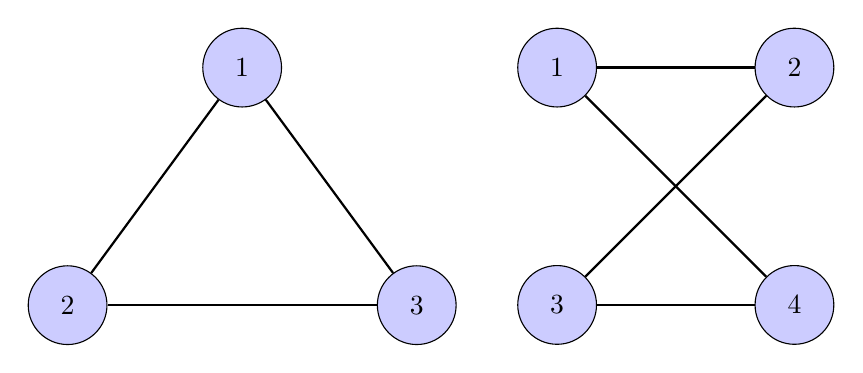
\begin{tikzpicture}
		\node[main node] (1) {$1$};
		\node[main node] (2) [below left = 2.3cm and 1.5cm of 1]  {$2$};
		\node[main node] (3) [below right = 2.3cm and 1.5cm of 1] {$3$};
		
		\path[draw,thick]
		(1) edge node {} (2)
		(2) edge node {} (3)
		(3) edge node {} (1);
		%%
		\begin{scope}[xshift=4cm]
			\node[main node] (1) {$1$};
			\node[main node] (2) [right = 2cm  of 1]  {$2$};
			\node[main node] (3) [below = 2cm  of 1] {$3$};
			\node[main node] (4) [right = 2cm  of 3] {$4$};
			
			\path[draw,thick]
			(1) edge node {} (2)
			(1) edge node {} (4)
			(3) edge node {} (2)
			(3) edge node {} (4)
			;
		\end{scope}
	\end{tikzpicture}
\caption{Egyszer\H u gr\'af TIKZ seg\'its\'eg\'evel}
\end{figure}




Továbbá megvalósítottam az Euler és Runge-Kutta módszerek párhuzamosított változatait is CUDA technológia segítségével. Ebben az esetben a tesztek azt mutatták, hogy az Euler módszer esetében többe kerül a sok CPU és GPU memória közötti másolás művelete, mint amennyit nyerünk a számítások elvégzése során. Tehát ebben az esetben ez a fajta párhuzamosítási megközelítés nem éri meg. Ezzel ellentétben a Runge-Kutta módszer esetében a megközelítés eredményesnek bizonyult abban az esetben, ha az egyenletek száma nagy és a lépésköz kicsi. A \ref{fejezet3_4} alfejezetben láthattuk, hogy abban az esetben ha az egyenletek száma $ n = 10 $ és a lépésköz $ h = 0.001 $, a GPU-n megközelítőleg 5 és fél perccel hamarabb lefutott az algoritmus, mint a CPU-n. Ezzel a párhuzamosítási módszerrel nem tudtuk kihasználni a videókártya által nyújtott maximális számítási kapacitást, de így is jelentős különbséget sikerült elérni a futási időket nézve, l\'asd \cite{Katai}.



	%----------------------------------------------------------------------------
\chapter{Tervezés	}
%----------------------------------------------------------------------------
Mindenképp egy blokkdiagrammal kell kezdeni, melyen a rendszer architektúráját ábrázoljuk. Az architektúra a rendszer lényeges komponenseit tartalmazza (hardver, szoftver, felhasználó, internet stb). Például lényeges, hogy a rendszerünk egy adatbázishoz kapcsolódik és mobilos interfésszel rendelkezik, nem lényeges vagy kevésbé lényeges, hogy milyen típusú adatbázist használ.

Itt el lehet indulni a \href{https://en.wikipedia.org/wiki/4\%2B1_architectural_view_model}{Krutchen} féle 4+1 architekturális nézetek iránya felé, mely szinten keretet ad a leírásnak. Érdemes a logikai (logical view) és a folyamat nézeteket (process view) leírni.

Szoftverfejlesztés esetében szoftver architektúráról van szó, melyet komponens diagram segítségével lehet a legjobban ábrázolni.  Amennyiben rendszerünk hardvert is tartalmaz ez is meg kell jelenjen az architektúrán.
Minden lényeges komponens szerepét pár mondatban le kell írni, hogy lehessen a rendszerről egy összképet alkotni. Esetenként pszeudokódot is lehet használni. Ebbe a fejezetbe nem kerül konkrét kód/kódrészlet. 

A szoftverrel kapcsolatos tervek után következhetnek (amennyiben van):
\begin{itemize}
\item Adatbázis terv
\item UI terv - pl. wireframe 
\item Extrák
			\begin{itemize}
			\item Verziókövetés pl. Github, egy branch vagy több. 
			\item Project management - pl. Kanban board segítségével követjük a taskokat.
			\item Rizikó elemzés és tesztelési terv.
		\end{itemize}
\end{itemize}
\begin{figure}[!h]
	\centering
	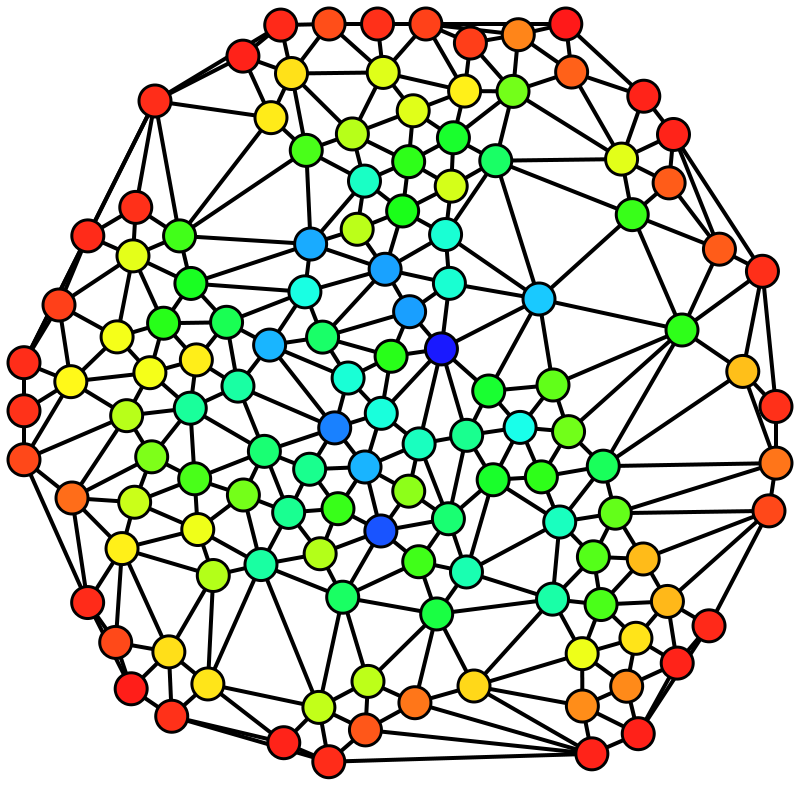
\includegraphics[scale=0.2]{images/graf1}
	\caption{Gr\'af}
\end{figure}


\begin{figure}[!h]
	\centering
	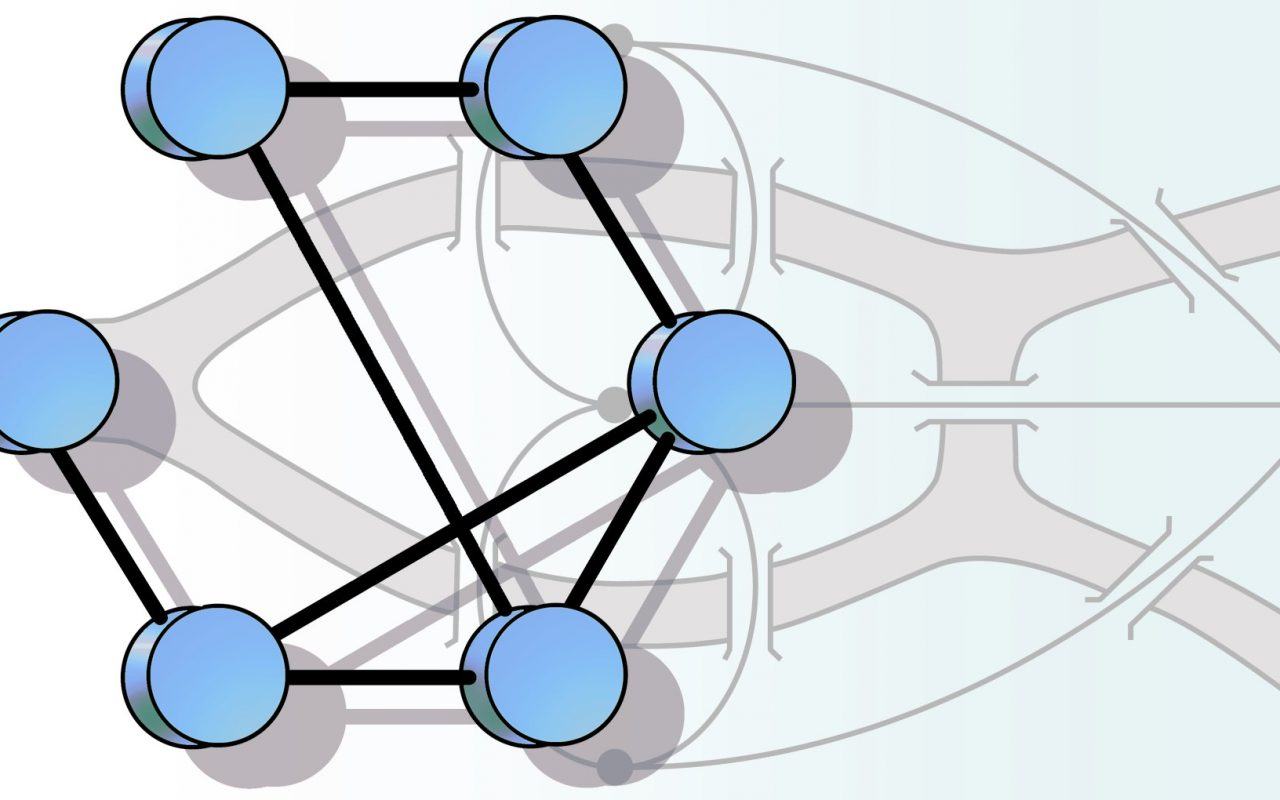
\includegraphics[scale=0.2]{images/graf2}
	\caption{Gr\'af 2}
\end{figure}


\begin{figure}[!h]
	\centering
	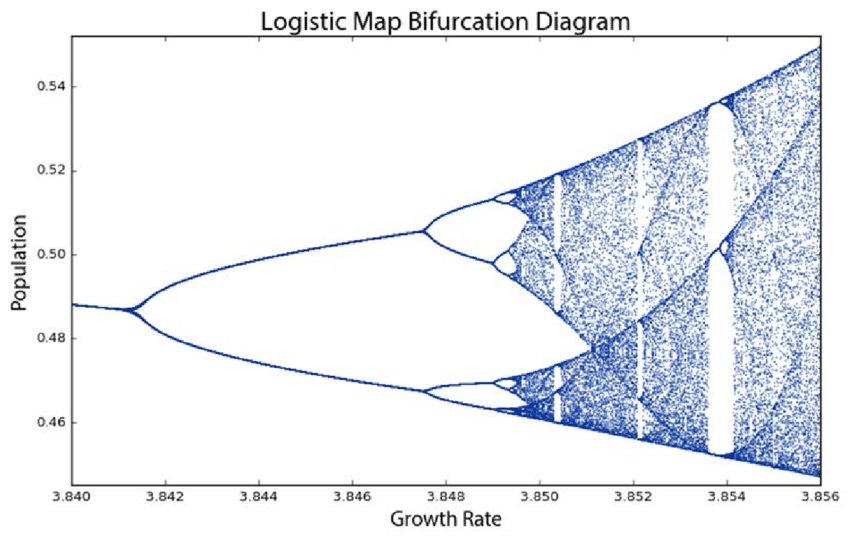
\includegraphics[scale=0.3]{images/kep2}
	\caption{Bifurk\'aci\'os diagram}
\end{figure}



\begin{figure}[!h]
	\centering
	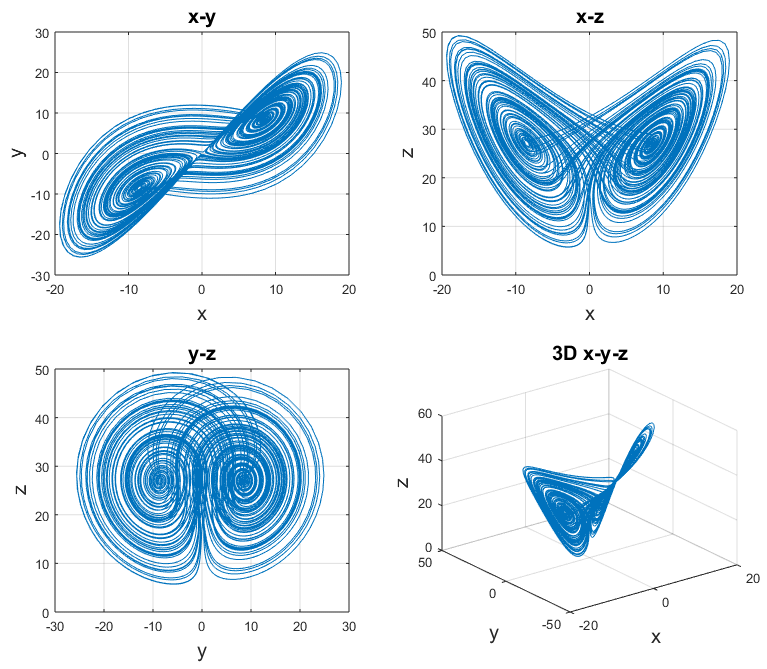
\includegraphics[scale=0.4]{images/kep33}
	\caption{Lorentz attraktor}
\end{figure}
	%----------------------------------------------------------------------------
\chapter{Kivitelezés}
%----------------------------------------------------------------------------


A megtervezett alkotás értékelése és kritikai elemzése.

Minden komponensre egy alfejezetet kell szánni, amelyben részletesen leírjuk a komponens belső működését, pl. osztálydiagramok segítségével.
Ha komponens más komponensekkel is kollaborál (igénybe veszi egy másik komponens publikus interface-ét vagy egy külső libraryt, függőséget/dependenciát használ), akkor ezt egy aktivitás-, vagy szekvencia diagrammal kell szemléltetni: pl. ki indítja a kommunikációt, mennyit vár, stb.


Ne próbáljunk egy diagrammal elintézni mindent. Érdemes egy használati esetre mint például a bejelentkezés vagy keresés egy-egy szekvencia diagramot készíteni. Annyi diagramot kell készíteni, amennyi elégséges ahhoz, hogy bemutassuk a rendszert. Figyelni kell, mert egyes diagramok a rendszer más-más aspektusait emelik ki (pl. Használati eset- és szekvencia diagram dinamikus képet, míg az osztálydiagram statikus képet ad a rendszerről).


Szoftverfejlesztés esetében ide lehet tenni a rendszerről készített képernyőképeket is. Lehet készíteni felhasználói útmutatót is. Érdemes csak a releváns részleteket bemutatni (nem releváns a bejelentkezés, releváns, hogy  mi történik a bejelentkezés után). A lényegesebb részeknél lehet konkrét kódrészletet is bemutatni. 





\section{P\'eld\'ak}

\begin{center}
	\begin{algorithm}[H]
		\KwIn{
			Integers $a \geq 0$ and $b \geq 0$}
		\KwOut{\textsc{Gcd} of $a$ and $b$} \While{$b \neq 0$}{
			$r \leftarrow a \bmod b$\;
			$a \leftarrow b$\;
			$b \leftarrow r$\;
		}
		\caption{Euclidean Algorithm}
	\end{algorithm}
\end{center}







\begin{algorithm}[H]
	\SetAlgoLined
	\KwData{this text}
	\KwResult{how to write algorithm with \LaTeX2e }
	initialization\;
	\While{not at end of this document}{
		read current\;
		\eIf{understand}{
			go to next section\;
			current section becomes this one\;
		}{
			go back to the beginning of current section\;
		}
	}
	\caption{How to write algorithms}
\end{algorithm}

\newpage
\begin{algorithm}[H]
	\DontPrintSemicolon
	\KwData{$G=(X,U)$ such that $G^{tc}$ is an order.}
	\KwResult{$G’=(X,V)$ with $V\subseteq U$ such that $G’^{tc}$ is an
		interval order.}
	\Begin{
		$V \longleftarrow U$\;
		$S \longleftarrow \emptyset$\;
		\For{$x\in X$}{
			$NbSuccInS(x) \longleftarrow 0$\;
			$NbPredInMin(x) \longleftarrow 0$\;
			$NbPredNotInMin(x) \longleftarrow |ImPred(x)|$\;
		}
		\For{$x \in X$}{
			\If{$NbPredInMin(x) = 0$ {\bf and} $NbPredNotInMin(x) = 0$}{
				$AppendToMin(x)$}
		}
		\nl\While{$S \neq \emptyset$}{\label{InRes1}
			\nlset{REM} remove $x$ from the list of $T$ of maximal index\;\label{InResR}
			\lnl{InRes2}\While{$|S \cap ImSucc(x)| \neq |S|$}{
				\For{$ y \in S-ImSucc(x)$}{
					\{ remove from $V$ all the arcs $zy$ : \}\;
					\For{$z \in ImPred(y) \cap Min$}{
						remove the arc $zy$ from $V$\;
						$NbSuccInS(z) \longleftarrow NbSuccInS(z) - 1$\;
						move $z$ in $T$ to the list preceding its present list\;
						\{i.e. If $z \in T[k]$, move $z$ from $T[k]$ to
						$T[k-1]$\}\;
					}
					$NbPredInMin(y) \longleftarrow 0$\;
					$NbPredNotInMin(y) \longleftarrow 0$\;
					$S \longleftarrow S - \{y\}$\;
					$AppendToMin(y)$\;
				}
			}
			$RemoveFromMin(x)$\;
		}
	}
	\caption{IntervalRestriction\label{IR}}
\end{algorithm}


Az általam írt szoftver egy \textbf{Java nyelv}en, \textbf{NetBeans IDE 8.0.1} fejlesztői környezetben írt asztali alkalmazás, amelynek fő funkcionalitása a kezdetiérték-probléma típusú differenciálegyenletek numerikus megoldása és ezen megoldások grafikus felületen való ábrázolása. A fő funkcionalitás mellett a szoftver tartalmaz még két kisebb funkcionalitást is, ezek közül az egyik a kétdimenziós függvényábrázolási lehetőség, a másik pedig a háromdimenziós függvények megjelenítésének lehetősége.

Az szoftver a differenciálegyenletek megoldásához a \ref{fejezet3}. fejezetben leírt numerikus eljárásokat alkalmazza.

A grafikus felhasználói felület megalkotásához a \textbf{Swing} (Java) komponens készletet használtam. A Swing használatával célom az volt, hogy egy felhasználóbarát és könnyen kezelhető felületet hozzak létre, amelyen a felhasználó könnyedén eligazodhat. Továbbá e komponenskészlet használata mellett szól az is, hogy a későbbiekben bemutatásra kerülő könyvtárak, melyek az ábrázolás megvalósítására használtam szintén Swing komponensekkel vannak megvalósítva.

Felhasználói felület, valamint a három funkcionalitás bemutatása képekben:

\begin{algorithm}[H]
	\Switch{order}{
		\uCase{bloody mary}{
			Add tomato juice\;
			Add vodka\;
			break\;
		}
		\uCase{hot whiskey}{
			Add whiskey\;
			Add hot water\;
			Add lemon and cloves\;
			Add sugar or honey to taste\; break\;
		}
		\Other{Serve wine\;}
	}
\caption{Switch haszn\'alata}
\end{algorithm}

\section {P\'elda 2}

	A szoftver elkészítésénél szükségem volt néhány előre megírt osztálykönyvtárra, amelyek megkönnyítették a munkámat. Ezekről tudni kell, hogy nyílt forráskódúak, tehát bárki számára elérhetőek az interneten, továbbá azt is, hogy ezek is Java nyelvben íródtak, hasonlóan, mint az általam írt alkalmazás. A továbbiakban szeretném bemutatni ezeket a könyvtárakat  és azt, hogy mire- és hogyan használtam fel őket.
	
	\begin{itemize}
		\item JMathPlot (\url{https://sites.google.com/site/mulabsltd/products/jmathplot}):
		\begin{itemize}
			\item Java könyvtár, amelyet interaktív megjelenítésre, ábrázolásra fejlesztettek
			\item gyors és könnyű utat biztosít tudományos adatok megjelenítésére Swing komponensek segítségével (nem használ openGL-t)
			\item az általa biztosított saját komponenseket úgy lehet használni, mint bármely más Swing komponenst
			\item a számomra legfontosabb tulajdonsága az, hogy két- és háromdimenziós ábrázolási lehetőséget biztosít, ezt használtam fel az alkalmazásomban
		\end{itemize}
		\item JMathArray (\url{https://sites.google.com/site/mulabsltd/products/jmatharray}):
		\begin{itemize}
			\item olyan Java könyvtár, amely alapvető matematikai, lineáris algebrai műveleteket biztosít számunkra 
			\item a könyvtár által biztosított statikus metódusok tömbökre alkalmazhatóak
			\item a szoftverben arra használtam, hogy egy megadott intervallum két végpontja között egy bizonyos lépésközzel haladva egy tömböt tudjak feltölteni (inkrementálás)
		\end{itemize}
		\item JEP (\url{http://www.cse.msu.edu/SENS/Software/jep-2.23/doc/website/}):
		\begin{itemize}
			\item szintén egy Java könyvtár, amelyet különböző elemzésekre és kiértékelésekre fejlesztettek
			\item segítségével egy szövegként (sztring-ként) megadott kifejezést könnyedén kiértékelhetünk, elvégezhetünk
			\item a szövegként megadott kifejezésből a háttérben egy kifejezésfát épít fel, majd a későbbiekben ennek a fának a segítségével dolgozik
			\item emellett sok általános matematikai függvény és konstans is bele van építve, amiket szintén könnyedén elérhetünk
			\item az általam fejlesztett szoftverben a függvények sztringként adhatók meg egy beviteli mezőn keresztül, a JEP könyvtárat ezen függvények „parszolására” használtam fel
%			\begin{figure}[h]
%				\centering
%				\includegraphics{figures/parszolas}
%				\caption{Egyszerű kifejezés elemzése, kiértékelése (Forrás: \url{http://www.singularsys.com/jep/doc/html/})}
%			\end{figure}
		\end{itemize}
	\end{itemize}


\subsection{Alfejezetekre p\'elda}
	A szoftver szerkezetileg két nagyobb részből (csomagból) áll, az egyik a felhasználói felület megalkotásához szükséges osztályokat tartalmazza, a másik pedig a differenciálegyenletek megoldására szolgáló osztályokat és a parszer osztályt, mely egy sztringként megadott függvény kiértékelésére szolgál.
	
	Az implementációnál a felhasználói felület elemeit tartalmazó csomagot „View”-nak, a numerikus módszereket és a parszert tartalmazó csomagot „Model”-nek neveztem, emellett a 6.7-es ábrán megjelenik egy harmadik csomag is, amely tartalmazza a „MainClass”-t és egyben a main() metódust is. Az alábbi két diagramon láthatjuk a felsorolt csomagokat és a bennük lévő osztályokat, illetve a köztük lévő kapcsolatokat.
	\pagebreak
	\begin{figure}
		\centering
		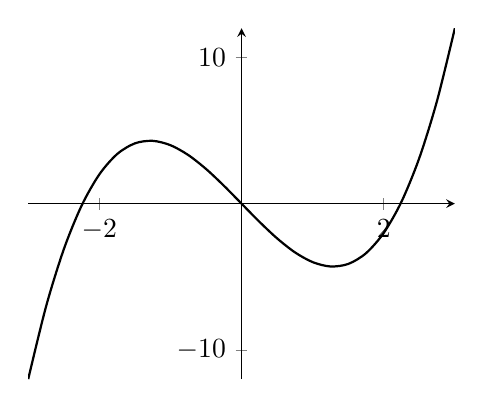
\begin{tikzpicture}
	\begin{axis} [axis lines=center]
		\addplot [domain=-3:3, smooth, thick] { x^3 - 5*x };
	\end{axis}
\end{tikzpicture}
\caption{Az $x^3-5x$ f\"uggv\'eny grafikus k\'epe PGFPLOT-al}
\end{figure}


\begin{figure}[h!]
	\centering
	\begin{tikzpicture}
		\begin{axis} [axis lines=center,xticklabels=\empty,yticklabels=\empty, xmin=-0.8,ymax=2.5,ytick style={draw=none}, xtick style={draw=none},tick,xlabel={$s$}]
			%N=6,p=3,p^*=6, p_*=5
			\addplot [domain=0:1, smooth, thick] { 1-2*x^(3) - 3*x^2  } node[midway,above right] {$\Psi$};
			\addplot[mark=*,color=red,] coordinates {(0.5,0)} node[midway,above right] {$\sigma^*$};
			\addplot[mark=*,color=red,] coordinates {(0,1)} node[midway,above left] {\scriptsize $\Psi(0)=\frac{1}{p2^{p-1}r_F^p}$};
		\end{axis}
	\end{tikzpicture}
	\caption{A $\Psi$ grafikus k\'epe}
\end{figure}
\pagebreak
\subsection{Alfejezet 2}
 \pgfplotsset{compat=1.11}
\begin{figure}[h!]
	\centering
	\begin{tikzpicture}[
		% define a style for the dots
		dot/.style={
			draw=black,
			fill=red!90,
			circle,
			minimum size=3pt,
			inner sep=0pt,
			solid,
		},
		]
		\begin{axis}[
			xmin=-1,
			xmax=2,
			ymin=-0.5,
			ymax=3,
			axis lines=center,
			ticks=none,
			xlabel={$s$},
			xlabel style={below right},
			ylabel style={above left},
			% (moved common `addplot' options here)
			smooth,
			domain=0:2,
			samples=101,
			no markers,
			draw=black
			]
			\addplot [blue,thick] {(9*x^(5/2)-x^(11/2)-2*x^(9/2))/(1+x^(3/2)+x^(7/2)) } node [midway,above right,color=black] {$\Lambda(s)$};
			\addplot[color=red,] coordinates {(0,0)} node[midway,above left] {$\Lambda(0)$};
			% draw the dots (using the above defined style) and labels
			\draw[dashed,color=red] (0.95,0) node [dot,label=below:$s_{\rm max}$] {}-- (0.95,2.017873338) node [dot,label=above:$\Lambda(s_{\rm max})$] {};
		\end{axis}
	\end{tikzpicture}
	\caption{A $\Lambda(s)$ grafikus k\'epe}\label{LAMBDA}
\end{figure}


\begin{figure}[!h]
	\centering
	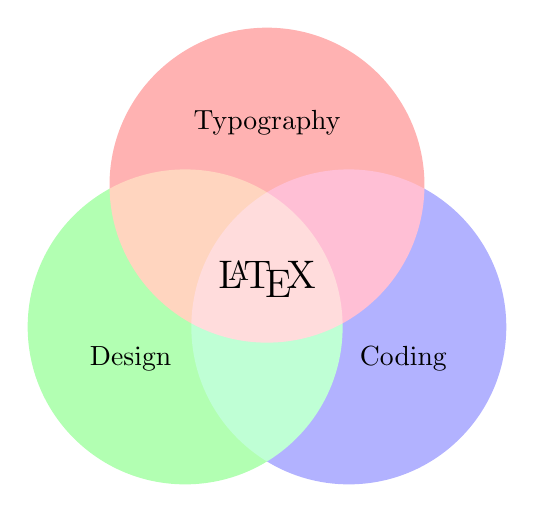
\begin{tikzpicture}
		\begin{scope}[blend group=soft light]
			\fill[red!30!white]   ( 90:1.2) circle (2);
			\fill[green!30!white] (210:1.2) circle (2);
			\fill[blue!30!white]  (330:1.2) circle (2);
		\end{scope}
		\node at ( 90:2) 	{Typography};
		\node at (210:2)  	{Design};
		\node at (330:2) {Coding};
		\node [font=\Large] {\LaTeX};
	\end{tikzpicture}
	\caption{Venn diagram TIKZ seg\'its\'egv\'evel}
\end{figure}


	\chapter{M\'er\'esek}

Csak kutatás-fejlesztéssel kapcsolatos dolgozat esetén. 

\section{P\'elda}

\begin{itemize}
	\item Futási idők \textbf{átlaga}: $ 0.0043 $ sec
	\item Futási idők \textbf{minimuma}: $ 0.0058 $ sec
	\item Futási idők \textbf{maximuma}: $ 0.0287 $ sec
\end{itemize}

A következő szoftvert, amit bemutatok \textbf{Java} nyelven írtam objektum orientáltan, a fejlesztés során pedig Eclipse fejlesztői környezetet használtam. Ez a szoftver három egységből áll: fő -, differenciálegyenlet megoldó - és kifejezés kiértékelő egység (ezt a legnehezebb megvalósítani vagy megtalálni a megfelelő könyvtárat). Az alkalmazás nem rendelkezik grafikus felhasználói felülettel, a bemeneti adatokat egy szöveges állományból olvassa be (amelynek jól meghatározott szerkezete van) és a kívánt eredményeket a standard kimenetre írja ki. A kifejezés kiértékelő egység megírásánál felhasználtam egy előre elkészített Java könyvtárat, melyet \href{http://www.singularsys.com/jep/}{\textit{JEP}}-nek neveznek. A szoftverben arra használtam fel, hogy egy sztringként megadott kifejezést kiértékeltem és elvégeztem a segítségével. Mindezt úgy csinálja, hogy a háttérben felépít egy kifejezésfát, aminek a leveleiben lesznek az értékek, csúcsaiban a műveletek, zárójelek, stb. (lásd az alábbi ábrát):



\begin{itemize}
	\item Futási idők \textbf{átlaga}: $ 0.1422 $ sec
	\item Futási idők \textbf{minimuma}: $ 0.123 $ sec
	\item Futási idők \textbf{maximuma}: $ 0.341 $ sec
\end{itemize}

Harmadiként lássuk a \textbf{C++ szoftvert}, amelyet szintén objektum orientáltam valósítottam meg. Ennek a szoftvernek a szerkezete hasonló a Java szoftver szerkezetéhez. Ebben az esetben is szükség volt egy kifejezés kiértékelő könyvtárra, hogy ne kelljen egy sajátot írni. Először kipróbáltam egy \href{http://beltoforion.de/article.php?a=muparser}{\textit{muparser}} nevű könytárat, aztán egy másikat is, aminek \href{https://exprtk.codeplex.com/}{\textit{ExprTk}} (Expression Toolkit Library) a neve. Fontos elmondani, hogy mindkét könyvtár ingyenesen elérhető és használható. Az első könyvtárat nehezebb volt hozzáadni a szoftverhez és mivel több fájlból állt több időbe került a fordítása is. A legfőbb ok, amiért mégis a másodikat használtam az volt, hogy jelentősen gyorsabb és hatékonyabb volt az én szoftveremben. Tehát végül az \textit{ExprTk} könyvtárat használtam a jobb teljesítménye és könnyebb integrálhatósága miatt.


\begin{itemize}
	\item Futási idők \textbf{átlaga}: $ 0.1086 $ sec
	\item Futási idők \textbf{minimuma}: $ 0.096 $ sec
	\item Futási idők \textbf{maximuma}: $ 0.214 $ sec
\end{itemize}

Végül nézzük meg az utolsó, Dormand-Prince módszeren alapuló szoftvert, amely egy \textbf{Android alkalmazás}. Mint tudjuk napjainkban a mobileszközök nagyon elterjedtek és teljesítményük is jelentősen megnőtt, lassan felveszik a versenyt a személyi számítógépekkel. Ezért mindenképp szerettem volna az algoritmust megvalósítani mobileszközökre is és megnézni itt is a teljesítményt. Mivel az Android alkalmazások fejlesztésénél Java nyelvet használunk, így könnyű dolgom volt, hiszen a Java szoftverből át tudtam venni a már jól megírt és elkülönített osztályokat. Ugyanazt a \textit{JEP} könyvtárat használtam itt is a kifejezések kiértékelésére, így majd az eredmények összehasonlítását is könnyebbé tettem. A Java és C++ szoftverrel ellentétben rendelkezik egy kis grafikus felhasználói felülettel, de a bemeneti adatokat itt is egy szöveges állományból olvassuk be, mert nem túl kényelmes azt a sok számadatot, meg egyenletet beviteli mezőkön keresztűl beírni.


\begin{itemize}
	\item Futási idők \textbf{átlaga}: $ 37.9015 $ sec
	\item Futási idők \textbf{minimuma}: $ 31.116 $ sec
	\item Futási idők \textbf{maximuma}: $ 70.876 $ sec
\end{itemize}


\section {Szoftverek összehasonlítása} \label{fejezet3_3}

Az előző alfejezetekben ismertettem a már létező Dormand-Prince módszeren alapú differenciálegyenlet megoldók közül kettőt és négy saját megvalósítást is. Mindegyik esetében láthattunk futási időket és számadatokat, azonban nem láttuk ezeket egymás mellett. Ebben az alfejezetben összegezzük és összehasonlítjuk a kapott eredményeket.

Fontos, hogy minden algoritmust ugyanazon a hardveren teszteljünk, mert csak így reálisak és összehasonlíthatóak a mérési adatok. Esetünkben használt hardver konfigurációja:
\begin{itemize}
	\item Intel Core i5-7200U, 2.50 GHz processzor, 8.00 GB RAM memória
\end{itemize}
Természetesen az Android alkamazást csak mobileszközökön lehetett vizsgálni, itt két készüléket használtam a tesztelésre:
\begin{itemize}
	\item Motorola Moto E2, Quad-core 1.2 GHz processzor, 1 GB RAM memória
	\item Samsung Galaxy Core Prime, Quad-core 1.2 GHz processzor, 1 GB RAM memória
\end{itemize}


\begin{table}[h!]
	\centering
	\begin{tabular}{ | l | c | c | c | c |}
		\hline 
		\textbf{Technológia} & \textbf{Átlagidő (s)} & \textbf{Min. idő (s)} & \textbf{Max. idő (s)} & \textbf{Hardver}\\
		\hline
		Matlab - ode45 & $ 0.0032 $ & $ 0.0029 $ & $ 0.0038 $ & Intel Core i5\\
		\hline
		Boost - Odeint & $ 0.0989 $ & $ 0.0900 $ & $ 0.1290 $ & Intel Core i5\\
		\hline
		Matlab & $ 0.0062 $ & $ 0.0060 $ & $ 0.0066 $ & Intel Core i5\\
		\hline
		Java & $ 0.2224 $ & $ 0.1970 $ & $ 0.3020 $ & Intel Core i5\\ 
		\hline
		C++ & $ 0.1047 $ & $ 0.1010 $ & $ 0.1240 $ & Intel Core i5\\
		\hline
		Android & $ 37.9015 $ & $ 31.1160 $ & $ 70.8760 $ & Moto E2\\
		\hline
		Android & $ 35.9987 $ & $ 29.4200 $ & $ 87.6120 $ & Core Prime\\
		\hline
	\end{tabular}
	\caption{Mérési eredmények  $ n = 10 $ tesztesetre.}
	\label{tablazat1}
\end{table}

\begin{table}[h!]
	\centering
	\begin{tabular}{ | l | c | c | c | c |}
		\hline 
		\textbf{Technológia} & \textbf{Átlagidő (s)} & \textbf{Min. idő (s)} & \textbf{Max. idő (s)} & \textbf{Hardver}\\
		\hline
		Matlab - ode45 & $ 0.0043 $ & $ 0.0026 $ & $ 0.1504 $ & Intel Core i5\\
		\hline
		Boost - Odeint & $ 0.0912 $ & $ 0.0900 $ & $ 0.0990 $ & Intel Core i5\\
		\hline
		Matlab & $ 0.0067 $ & $ 0.0058 $ & $ 0.0287 $ & Intel Core i5\\
		\hline
		Java & $ 0.1422 $ & $ 0.1230 $ & $ 0.3410 $ & Intel Core i5\\ 
		\hline
		C++ & $ 0.1086 $ & $ 0.0960 $ & $ 0.2140 $ & Intel Core i5\\
		\hline
		Android & $ - $ & $ - $ & $ - $ & Moto E2\\
		\hline
		Android & $ - $ & $ - $ & $ - $ & Core Prime\\
		\hline
	\end{tabular}
	\caption{Mérési eredmények  $ n = 100 $ tesztesetre.}
\end{table}



\label{fejezet3_4}


A továbbiakban nézzük meg a két algoritmus magjának szekvenciális és párhuzamosított változatait:
\begin{lstlisting}[caption={Euler módszer szekvenciális kód.}, captionpos=b, language = C++]
	for (int i = 0; i < numberOfVariables; ++i) {
		mResult.at(i)[j + 1] = mResult.at(i)[j] + mInputs->getStepSize() *
		(mFunctionsParsers.at(i)->computeFunctionValue(values));
	}
\end{lstlisting}

\begin{lstlisting}[caption={Euler módszer párhuzamosított kód.}, captionpos=b, language = C++]
	__global__ void computeFunctionsValuesKernel(double* resultValues,
	double* previousValues, double* functionValues, double stepSize, int N) {
		int i = threadIdx.x;
		
		if (i < N) {
			resultValues[i] = previousValues[i] + stepSize * functionValues[i];
		}
	}
\end{lstlisting}

\begin{lstlisting}[caption={Runge-Kutta módszer szekvenciális kód.}, captionpos=b, language = C++]
	for (int k = 0; k < numberOfVariables; ++k) {
		mResult.at(k)[i + 1] = mResult.at(k)[i] + (mInputs->getStepSize() / 6)*
		(K[0][k] + 2 * K[1][k] + 2 * K[2][k] + K[3][k]);
	}
\end{lstlisting}

\begin{lstlisting}[caption={Runge-Kutta módszer párhuzamosított kód.}, captionpos=b, language = C++]
	__global__ void computeValuesKernel(double* resultValues, double* K,
	double* previousValues, double stepSize, int numberOfVariables) {
		int i = threadIdx.x;
		
		if (i < numberOfVariables) {
			resultValues[i] = previousValues[i] + ((stepSize / 6) *
			(K[i] + 2 * K[i + 1 * numberOfVariables] +
			2 * K[i + 2 * numberOfVariables] + K[i + 3 * numberOfVariables]));
		}
	}
\end{lstlisting}

Nézzünk meg pár mérési eredményt a következő differenciálegyenlet rendszerre:
\begin{align}
	\begin{cases}
		y_{1}'(t, y) = y_{1} \\
		\vdots \\
		y_{n}'(t, y) = y_{n}\\
		y_{1}'(t_{0}) = 1.0 \\
		\vdots \\
		y_{n}'(t_{0}) = 1.0\\
	\end{cases}
	, t\in[0, 100], n = 5
\end{align}

\begin{table}[h!]
	\centering
	\begin{tabular}{ | p{1.8cm} | p{2.5cm} | p{2.5cm} | p{2.5cm} | p{2.5cm} |}
		\hline  & \multicolumn{2}{|c|}{\textbf{CPU sec (Intel Core i5)}} & \multicolumn{2}{|c|}{\textbf{GPU sec (GeForce 940MX)}}\\ 
		\hline  & Euler & Runge-Kutta & Euler & Runge-Kutta\\ 
		\hline
		$ h = 10.0 $ & $ 0.006 $ & $ 0.036 $ & $ 0.587 $ & $ 0.036 $ \\ 
		\hline
		$ h = 1.0 $ & $ 0.074 $ & $ 0.523 $ & $ 0.841 $ & $ 0.490 $ \\
		\hline
		$ h = 0.1 $ & $ 0.689 $ & $ 4.987 $ & $ 1.565 $ & $ 3.399 $ \\
		\hline
		$ h = 0.01 $ & $ 7.202 $ & $ 52.800 $ & $ 14.321 $ & $ 50.110 $ \\
		\hline
		$ h = 0.001 $ & $ 71.071 $ & $ 500.999 $ & $ 98.445 $ & $ 321.965 $ \\
		\hline
	\end{tabular}
	\caption{Mérési eredmények $ n = 5 $ egyenlet esetén.}
\end{table}

\begin{align}
	\begin{cases}
		y_{1}'(t, y) = y_{1} \\
		\vdots \\
		y_{n}'(t, y) = y_{n}\\
		y_{1}'(t_{0}) = 1.0 \\
		\vdots \\
		y_{n}'(t_{0}) = 1.0\\
	\end{cases}
	, t\in[0, 100], n = 10
\end{align}

\begin{table}[h!]
	\centering
	\begin{tabular}{ | p{1.8cm} | p{2.5cm} | p{2.5cm} | p{2.5cm} | p{2.5cm} |}
		\hline  & \multicolumn{2}{|c|}{\textbf{CPU sec (Intel Core i7)}} & \multicolumn{2}{|c|}{\textbf{GPU sec (GeForce 950M)}}\\ 
		\hline  & Euler & Runge-Kutta & Euler & Runge-Kutta\\ 
		\hline
		$ h = 10.0 $ & $ 0.039 $ & $ 0.256 $ & $ 1.070 $ & $ 0.222 $ \\ 
		\hline
		$ h = 1.0 $ & $ 0.320 $ & $ 2.482 $ & $ 0.994 $ & $ 2.087 $ \\
		\hline
		$ h = 0.1 $ & $ 3.042 $ & $ 23.962 $ & $ 4.143 $ & $ 20.978 $ \\
		\hline
		$ h = 0.01 $ & $ 30.812 $ & $ 241.977 $ & $ 35.009 $ & $ 206.842 $ \\
		\hline
		$ h = 0.001 $ & $ 305.092 $ & $ 2394.930 $ & $ 344.485 $ & $ 2067.870 $ \\
		\hline
	\end{tabular}
	\caption{Mérési eredmények $ n = 10 $ egyenlet esetén.}
\end{table}
	%----------------------------------------------------------------------------
\chapter*{Összefoglaló}\addcontentsline{toc}{chapter}{Összefoglaló}
%----------------------------------------------------------------------------


Ez a fejezet röviden összefoglalja a dolgozatot. Leírja a dolgozatból levonható általános következtetéseket. Ugyanakkor itt lehet megfogalmazni a jövőbeli terveket, további fejlesztési lehetőségeket.

Kötelező megadni a publikus Git Repository-t (GitHub, GitLab). 







\section{P\'elda}
Dolgozatomban differenciálegyenletek megoldásával foglalkoztam, amelyet különböző programozási technológiák segítségével valósítottam meg. Először ismertettem a differenciálegyenletek numerikus megoldásának elméleti alapjait, majd megvizsgáltunk és levezettünk három numerikus módszert az Euler-, a Runge-Kutta és a Dormand-Prince módszereket. Ezek közül a mai technológiákban leginkább használatos Dormand-Prince algoritmus esetében megnéztük, hogy milyen szoftverekben tálálhatjuk meg, mint alapértelmezett differenciálegyenlet megoldó. A továbbiakban ismertettem két modellt, a leukémia betegség alap modelljét és a hullámmozgás modelljét, ezzel is kihangsúlyozva a téma fontosságát, hogy mennyire fontos az időtényező bizonyos problémák egyenleteinek medoldásánál. Ezek után részletesen is mégnéztük, hogy milyen szoftvereket alkalmaztam és alkottam a differenciálegyenletek és rendszerek megoldására. A szoftvereket két kategóriába osztotottuk fel, az első a már létező szoftverek kategóriája, a másik pedig az általam megvalósított szoftverek csoportja volt. Az első kategóriában ismertettem két technológiát, a Matlab által nyúltott ode45 beépített megoldót és a Boost könyvtárcsomagban található Odeint nevű könyvtárat. Az általam írt szofverek csoportjában négy megvalósítást mutattam be ezek a Matlab, Java, C++ és Android technológiák segítségével készültek. Emellett megnéztük, hogy mennyire hatékonyan lehet párhuzamosítani a differenciálegyenletek megoldását CUDA technológia segítségével és a grafikus kártyát (GPU-t) felhasználva. Végül kiértékeltük a tesztelés során kapott eredményeket és összehasonlítottuk a különböző programokat, kiemelve azok erősségeit és gyengéit. Majd levontuk a következtetéseket, hogy melyik technológia irányában érdemes tovább haladni és melyik az, amelyikkel nem éri meg foglalkozni.

Jövőbeli terveimet illetően szeretnék jobban elmerülni a GPU-n történő differenciálegyenletek megoldásának módszereiben, valamint ezek alkalmazását kipróbálni és tanulmányozni a parciális differenciálegyenletek területén (PDE). Továbbá érdemesnek tartom a C++ szoftver továbbfejlesztését és egy differenciálegyenlet megoldó könyvtár megalkotását, amely ingyenesen használható és nyílt forráskódú lenne.

% Koszonetnyilvanitas
%~~~~~~~~~~~~~~~~~~~~~~~~~~~~~~~~~~~~~~~~~~~~~~~~~~~~~~~~~~~~~~~~~~~~~~~~~~~~~~~~~~~~~~
	%----------------------------------------------------------------------------
\chapter*{\koszonetnyilvanitas}\addcontentsline{toc}{chapter}{\koszonetnyilvanitas}
%----------------------------------------------------------------------------

Ez nem kötelező, akár törölhető is. Ha a szerző szükségét érzi, itt lehet köszönetet nyilvánítani azoknak, akik hozzájárultak munkájukkal ahhoz, hogy a hallgató a szakdolgozatban vagy diplomamunkában leírt feladatokat sikeresen elvégezze. A konzulensnek való köszönetnyilvánítás sem kötelező, a konzulensnek hivatalosan is dolga, hogy a hallgatót konzultálja.


% Tablazatok es abrak jegyzeke (EZ NEM KOTELEZO)
%~~~~~~~~~~~~~~~~~~~~~~~~~~~~~~~~~~~~~~~~~~~~~~~~~~~~~~~~~~~~~~~~~~~~~~~~~~~~~~~~~~~~~~
	\listoffigures\addcontentsline{toc}{chapter}{\abrakjegyzeke}
	\listoftables\addcontentsline{toc}{chapter}{\tablazatokjegyzeke}


% Bibliography
%~~~~~~~~~~~~~~~~~~~~~~~~~~~~~~~~~~~~~~~~~~~~~~~~~~~~~~~~~~~~~~~~~~~~~~~~~~~~~~~~~~~~~~
	\bibliography{mybib}
	\addcontentsline{toc}{chapter}{\irodalomjegyzek}
	\bibliographystyle{alpha}
	
% Appendix
%~~~~~~~~~~~~~~~~~~~~~~~~~~~~~~~~~~~~~~~~~~~~~~~~~~~~~~~~~~~~~~~~~~~~~~~~~~~~~~~~~~~~~~
	%----------------------------------------------------------------------------
\appendix
%----------------------------------------------------------------------------
\chapter*{\fuggelek}\addcontentsline{toc}{chapter}{\fuggelek}
\setcounter{chapter}{6}  % a fofejezet-szamlalo az angol ABC 6. betuje (F) lesz
\setcounter{equation}{0} % a fofejezet-szamlalo az angol ABC 6. betuje (F) lesz
\numberwithin{equation}{section}
\numberwithin{figure}{section}
\numberwithin{lstlisting}{section}
%\numberwithin{tabular}{section}

%----------------------------------------------------------------------------
\section{A TeXstudio felülete}
%----------------------------------------------------------------------------
\begin{figure}[!ht]
\centering
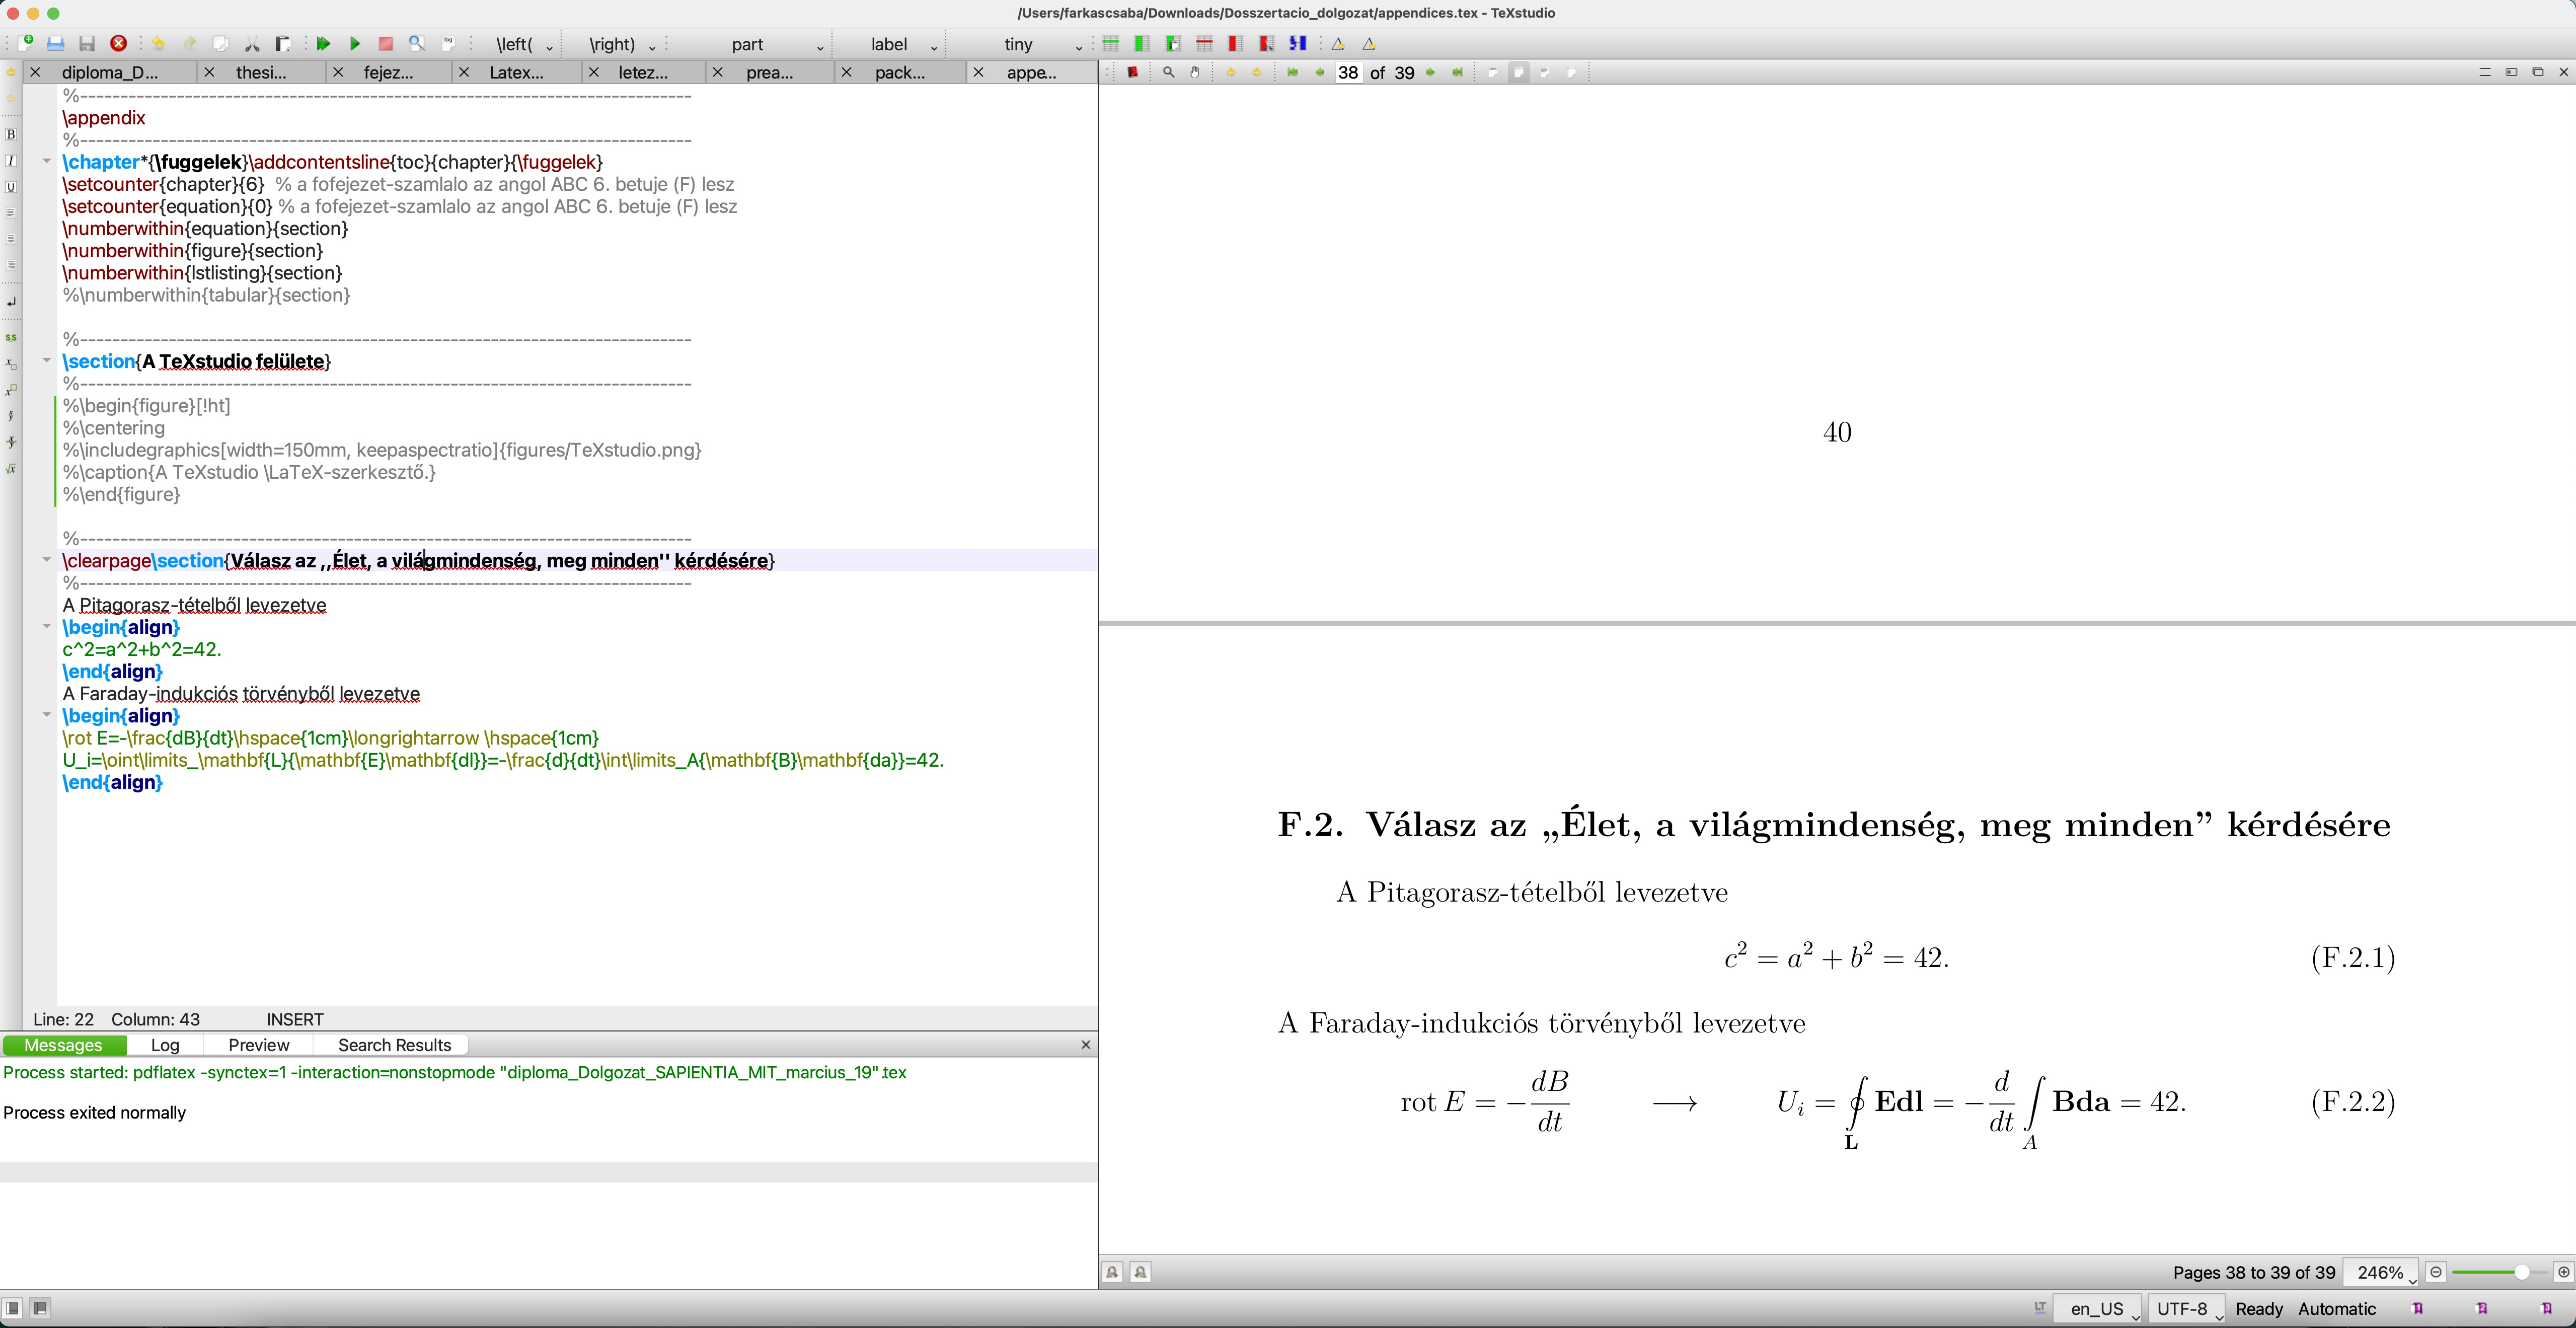
\includegraphics[width=150mm, keepaspectratio]{images/texstudio}
\caption{A TeXstudio \LaTeX-szerkesztő.} 
\end{figure}

%----------------------------------------------------------------------------
\clearpage\section{Válasz az ,,Élet, a világmindenség, meg minden'' kérdésére}
%----------------------------------------------------------------------------
A Pitagorasz-tételből levezetve
\begin{align}
c^2=a^2+b^2=42.
\end{align}
A Faraday-indukciós törvényből levezetve
\begin{align}
\rot E=-\frac{dB}{dt}\hspace{1cm}\longrightarrow \hspace{1cm}
U_i=\oint\limits_\mathbf{L}{\mathbf{E}\mathbf{dl}}=-\frac{d}{dt}\int\limits_A{\mathbf{B}\mathbf{da}}=42.
\end{align}







\label{page:last}
\end{document}
